\documentclass[12pt, a4paper, twoside]{article}

\usepackage{fancyhdr}
\fancyhfoffset{0pt}
\usepackage{pdfpages}
\usepackage[magyar]{babel}
\usepackage{titlesec}
\usepackage{fontspec}
\usepackage{float}

% Betűtípusok
\setmainfont{Times New Roman}[
    WordSpace = 1.2
]

\newfontfamily\headingFont{Arial}[
    WordSpace = 1.2
]

% Fejezetcímek
\newcommand{\sectionbreak}{\clearpage}

\titleformat{\section}
    {\headingFont\bfseries\fontsize{16}{24}\selectfont}
    {\thesection}
    {1em}
    {}

\titlespacing*{\section}
    {0pt}
    {0pt}
    {12pt}

\titleformat{\subsection}
    {\headingFont\bfseries\fontsize{14}{14}\selectfont}
    {\thesubsection}
    {1em}
    {}

\titlespacing*{\subsection}
    {0pt}
    {12pt}
    {12pt}

\titleformat{\subsubsection}
    {\headingFont\bfseries\fontsize{12}{12}\selectfont}
    {\thesubsubsection}
    {1em}
    {}

\titlespacing*{\subsubsection}
    {0pt}
    {12pt}
    {6pt}

% Élőfej és élőláb
\pagestyle{fancy}
\fancyhf{}
\renewcommand{\headrulewidth}{0pt}
\renewcommand{\footrulewidth}{0pt}
\fancyfoot[EL,OR]{\thepage}

% Oldalelrendezés, ábrák, táblázatok
\usepackage{multirow}
\usepackage[margin=2.5cm]{geometry}
\usepackage{graphicx}
\usepackage{amsmath}
\usepackage{caption}
\usepackage{tikz}
\usetikzlibrary{positioning,arrows.meta}
\usepackage{array}
\usepackage{longtable}
\usepackage{booktabs}

\captionsetup{
    labelfont=bf,
    labelsep=colon,
    font=footnotesize
}

% Listák és sortávolság
\usepackage{enumitem}
\setlist[itemize]{label=--}

\usepackage{setspace}
\setstretch{1.5}

\setlength{\parindent}{0pt}
\usepackage{parskip}
\setlength{\parskip}{6pt}

% Irodalomjegyzék
\usepackage[square, numbers]{natbib}

\begin{document}

% Címlap
\begin{titlepage}
    \centering
    \vspace*{1cm}

    {\Huge \bfseries Hibabejelentő és karbantartás-kezelő
    rendszer \par}

    \vspace{2.5cm}

    {\Large \textbf{Szerzők:}\par}
    \vspace{0.2cm}
    {\large Farkas Levente, Horváth Dániel, Kantó József\par}

    \vspace{2cm}

    {\Large \textbf{Témavezető:}\par}
    \vspace{0.2cm}
    {\large Dr. Tarczali Tünde Tímea, adjunktus\par}

    \vfill
    {\large 2026\par}
\end{titlepage}

% Ha szükség van üres hátoldalra, később külön PDF-fájlként
% feltölthető és itt visszaállítható az includepdf parancs.

\newpage
\pagenumbering{gobble}

% Kivonat
\begin{center}
    \noindent
    {\headingFont\bfseries\fontsize{16}{24}\selectfont Kivonat}
\end{center}
\addcontentsline{toc}{section}{Kivonat}
\vspace{12pt}

A projekt célja egy olyan asztali hibabejelentő és karbantartás-kezelő rendszer megtervezése és fokozatos megvalósítása, amely támogatja egy szervezet műszaki, jelen projektben elsősorban informatikai hibáinak bejelentését és kezelését. A rendszerben a felhasználók bejelentéseket hozhatnak létre, követhetik azok állapotát, a karbantartók pedig a csoportjukhoz rendelt feladatokat vehetik fel és kezelhetik.

A rendszer tervezése során meghatároztuk a fő felhasználói szerepköröket, a bejelentések kezelésének folyamatát, valamint az alkalmazás alapvető architektúráját. A megvalósított megoldás .NET MAUI asztali kliensből, .NET Web API-ból és a szerveroldalon kezelt SQLite-adatbázisból áll. A kliens HTTP-kéréseken keresztül kommunikál a szerverrel, az üzleti logikát és az adatbázis-hozzáférést pedig a Web API kezeli.

A backend tartalmazza a regisztrációt és a bejelentkezést, a JWT-alapú hitelesítést, a jogosultságok ellenőrzését, a hibajegyek teljes életciklusát -- létrehozás, adminisztrátori elfogadás, karbantartói felvétel, kommunikációs bejegyzések, automatikus státuszkezelés, lezárás, újranyitás és visszavonás --, a státuszelőzmények lekérdezését, valamint a csoportok, kategóriák, helyszínek és prioritások adminisztrációját. A kliensben jelenleg a bejelentkezés, a hibajegylista keresése és szűrése, a hibajegy adatainak megjelenítése és új hibajegy létrehozása érhető el. Az értesítési rendszer és a bővített szerveroldali keresés még hátralévő feladat.

\textbf{Kulcsszavak:} hibabejelentés, ticketkezelés, .NET MAUI, Web API, SQLite, JWT

\newpage
\tableofcontents

\newpage
\pagenumbering{arabic}
\setcounter{page}{1}

\section{Bevezetés}

Egy szervezet mindennapi működését különböző műszaki problémák nehezíthetik. Ezek között lehetnek épülethez, eszközökhöz, hálózathoz vagy informatikai szolgáltatásokhoz kapcsolódó hibák. Ha a problémák bejelentése informális csatornákon, például szóban vagy e-mailben történik, nehezebb nyomon követni, hogy ki foglalkozik velük, milyen állapotban vannak, és milyen intézkedés történt.

A projekt célja egy olyan alkalmazás megtervezése és megvalósítása, amely egységes felületet biztosít a hibák bejelentésére, nyilvántartására és kezelésére. A bejelentő rögzítheti a probléma lényeges adatait, később megtekintheti saját bejelentéseinek állapotát, a karbantartást végző munkatárs pedig felveheti és kezelheti a csoportjához rendelt feladatokat.

A kiadott projektfeladat általános műszaki hibabejelentő rendszert ír le. A projekt jelenlegi terve ezt a feladatot egy szervezet belső, elsősorban informatikai infrastruktúrájához kapcsolódó hibakezelési folyamatára szűkíti. A dokumentációban ezt a szűkített projektkört használjuk.

\subsection{A projekt célja}

A rendszer célja, hogy a hibabejelentések kezelése átlátható, visszakereshető és szerepkörökhöz kötött legyen. A bejelentéseknek egyedi azonosítójuk van, és az életciklusuk során rögzülnek a hozzájuk tartozó állapotváltozások és kommunikációs bejegyzések.

A rendszer fő funkciói:

\begin{itemize}
    \item műszaki hibák bejelentése;
    \item egyedi azonosító rendelése a bejelentésekhez;
    \item a bejelentések kategorizálása és priorizálása;
    \item bejelentések karbantartói csoporthoz rendelése;
    \item a csoporttagok számára a csoporthoz rendelt feladatok megtekintése;
    \item a feladatok felvétele és kezelése;
    \item a bejelentés állapotának követése és az állapotváltozások előzményeinek megőrzése;
    \item kommunikációs bejegyzések és javítási információk rögzítése;
    \item lezárás típus szerint, illetve indoklással történő újranyitás;
    \item alkalmazáson belüli értesítések megjelenítése (tervezett);
    \item felhasználók, csoportok, kategóriák, helyszínek és prioritások adminisztrációja.
\end{itemize}

\subsection{A projekt hatóköre}

A projekt első változata a bejelentés létrehozására, nyomon követésére és kezelésére összpontosít. A rendszer felhasználói bejelentői, karbantartói és adminisztrátori feladatokat látnak el. A karbantartó nem külön felhasználói típus: a karbantartói feladatokat olyan felhasználó végzi, aki egy karbantartói csoport tagja.

A backend jelenleg az egyedi ticketazonosító alapján tud egy konkrét hibajegyet lekérni, a listázó végpontok pedig a felhasználóhoz tartozó teljes listát adják vissza. A kliens ezen a listán belül szöveges keresést és állapot szerinti szűrést biztosít. A kategória, prioritás vagy dátum szerinti szerveroldali szűrés, illetve a bővített keresés későbbi bővítésként szerepel. E-mailes értesítés nem része az első változat követelményeinek; a rendszer alkalmazáson belüli értesítéseket tervez, ezek megvalósítása még hátravan.

\subsection{A projekt tervezése}

A munka a kiadott specifikáció elemzésével kezdődött. A csapat meghatározta a fő funkciókat, a felhasználói szerepköröket, valamint a bejelentések kezelésének alapvető folyamatát. A tervezéshez használati eseteket és adatbázistervet készítettünk.

A rendszer központi eleme a hibabejelentés, más néven ticket. A felhasználó létrehozza a bejelentést, az adminisztrátor elfogadja, szükség esetén módosítja a kategóriáját, prioritást rendel hozzá, majd karbantartói csoporthoz rendeli. A csoport tagjai megtekintik a feladatot, és egyikük felveheti annak kezelését. A felvevő karbantartó és a bejelentő bejegyzésekben kommunikál egymással; a bejegyzések automatikusan módosítják a jegy állapotát. A karbantartó végső bejegyzéssel és lezárási típussal zárja le a bejelentést, a bejelentő pedig indoklással újranyithatja a lezárt jegyet.

\section{Követelmények és szerepkörök}

\subsection{Felhasználói szerepkörök}

A rendszer három fő szerepkört különít el: bejelentő, karbantartó és adminisztrátor. A jogosultságok meghatározzák, hogy az adott felhasználó mely bejelentéseket láthatja, illetve milyen műveleteket hajthat végre. A szerepkörök nem zárják ki egymást: minden jóváhagyott felhasználó bejelentő, a csoporttagság karbantartói, az \texttt{IsAdmin} jelző pedig adminisztrátori jogokat ad.

\subsubsection{Felhasználó és hibabejelentő}

A hibabejelentő a rendszer alapvető felhasználója. Regisztráció és adminisztrátori jóváhagyás után bejelentkezhet az alkalmazásba. Új hibabejelentést hozhat létre, megtekintheti saját bejelentéseit, és egyedi azonosító alapján lekérheti azokat.

A bejelentő kommunikációs bejegyzést írhat a saját ticketjéhez, ha az nincs lezárva vagy visszavonva. Ezt már az adminisztrátori elfogadás előtt, \textit{Új} állapotban is megteheti, például kiegészítő információ megadására. A lezárt bejelentését indoklással újranyithatja, saját hibajegyét pedig bármikor visszavonhatja.

\subsubsection{Karbantartó}

A karbantartó olyan felhasználó, aki egy aktív karbantartói csoport tagja. A csoporthoz rendelt ticketeket külön listában megtekintheti, és a csoport tagjaként magára veheti valamelyik, még fel nem vett feladatot. Egy ticketet egyszerre csak egy karbantartó vehet fel.

A felvett ticketen a karbantartó bejegyzést írhat a bejelentőnek, majd a munka végén végső bejegyzéssel és lezárási típussal lezárhatja a feladatot. A csoport többi tagja a ticketet és a bejegyzéseket látja, de bejegyzést csak a felvevő karbantartó írhat. A karbantartó a bejelentői funkciókat is használhatja, tehát saját maga is létrehozhat hibabejelentést.

\subsubsection{Rendszeradminisztrátor}

Az adminisztrátor felelős a rendszer alapadatainak és felhasználóinak kezeléséért. Jóváhagyhatja a regisztrációkat, inaktiválhat felhasználókat, csoporthoz rendelheti őket, valamint kezelheti a karbantartói csoportokat, a kategóriákat, a helyszíneket és a prioritásokat.

Az adminisztrátor áttekintheti az összes hibajegyet, az új hibajegyeket elfogadhatja, és az elfogadás során beállíthatja a kategóriát, a prioritást és a felelős karbantartói csoportot. Az adminisztrátori fiók külön jogosultsági kategória; az adminisztrátori felhasználó nem kerül automatikusan karbantartói csoportba.

A prioritások nevét és a hozzájuk tartozó munkanapos határidőt az adminisztrátor az alkalmazás adatai között kezeli; ezek nem a forráskódban rögzített értékek.

\subsection{Regisztráció és felhasználókezelés}

A regisztrációs folyamat lépései:

\begin{enumerate}
    \item A felhasználó regisztrációt kezdeményez névvel, e-mail-címmel és jelszóval.
    \item A regisztráció adminisztrátori jóváhagyásra vár.
    \item Az adminisztrátor áttekinti a regisztrációt.
    \item Jóváhagyás után a felhasználó aktívvá válik.
    \item Az aktív, jóváhagyott felhasználó bejelentkezhet az alkalmazásba.
\end{enumerate}

A regisztráció és a bejelentkezés külön funkció. A regisztráció felhasználói fiókot kezdeményez, a bejelentkezés pedig egy már jóváhagyott fiók használatát teszi lehetővé. A név 2--100, a jelszó legalább 8 karakter hosszú lehet, az e-mail-cím pedig legfeljebb 150 karakteres és egyedi.

A jelenlegi követelmények szerint a felhasználó manuális létrehozása, általános adatainak módosítása és törlése nem része az adminisztrátori funkcióknak. A felhasználó inaktiválható, jóváhagyható, illetve karbantartói csoporthoz rendelhető vagy onnan eltávolítható. Egy felhasználó legfeljebb egy karbantartói csoport tagja lehet. Az utolsó aktív adminisztrátor nem inaktiválható, egy csoport pedig csak akkor inaktiválható, ha már nincs aktív tagja.

\subsection{Bejelentések adatai}

A bejelentés az alábbi adatokat tartalmazza:

\begin{itemize}
    \item egyedi ticketazonosító;
    \item cím és leírás;
    \item kötelező helyszín, amely az adminisztrátor által kezelt helyszínlistából választható;
    \item opcionális eszközazonosító;
    \item kategória;
    \item prioritás;
    \item határidő;
    \item aktuális állapot;
    \item bejelentő;
    \item hozzárendelt karbantartói csoport;
    \item a ticketet felvevő karbantartó, ha már valaki felvette a feladatot;
    \item a bejelentéshez tartozó bejegyzések és státuszelőzmények;
    \item létrehozás, módosítás és lezárás időpontja.
\end{itemize}

A bejelentés helyszínének megadása kötelező, mert ez segíti a hiba beazonosítását és a szükséges intézkedés megtervezését. A helyszín nem szabad szövegként, hanem az aktív helyszínek egyikeként adható meg, így az azonos helyszínek egységesen jelennek meg. Az érintett eszköz azonosítója opcionális, mivel nem minden probléma köthető egy konkrét eszközhöz.

A prioritás az adminisztrátor által kezelt prioritáslista egyik eleme. Minden prioritáshoz tartozik egy munkanapban megadott határidő, és pontosan egy aktív prioritás jelölhető alapértelmezettnek. A bejelentő nem választ prioritást: az új ticket az alapértelmezett prioritást kapja, a végleges prioritást pedig az adminisztrátor állítja be az elfogadáskor. A kezdeti adatbázisban négy prioritás szerepel: Sürgős 1, Magas 3, Normál 5 és Alacsony 10 munkanappal; ezek közül a Normál az alapértelmezett.

A határidő munkanapokban számítódik. Az első változatban munkanapnak a hétfőtől péntekig tartó napok számítanak; a munkaszüneti napok külön naptári kezelése nem része a rendszernek. A határidő a bejelentés létrehozásakor az alapértelmezett prioritás alapján keletkezik, majd az adminisztrátori elfogadáskor az akkor kiválasztott prioritás alapján, az elfogadás időpontjától újraszámolódik.

A kategóriák adminisztrátori kezelés alatt állnak. A kategória azt jelöli, hogy a probléma milyen jellegű, és így melyik kezelési területhez tartozik. A bejelentő a létrehozáskor kategóriát választ, amelyet az adminisztrátor az elfogadáskor módosíthat.

\subsection{Állapotok és munkafolyamat}
\label{sec:states}

A bejelentés lehetséges állapotai:

\begin{itemize}
    \item \textbf{Új:} a ticket létrejött, adminisztrátori elfogadásra vár;
    \item \textbf{Folyamatban:} a ticketet az adminisztrátor elfogadta és csoporthoz rendelte, vagy a bejelentő válaszolt a karbantartónak;
    \item \textbf{Válaszra vár:} a felvevő karbantartó bejegyzést írt, a bejelentő reakciója szükséges;
    \item \textbf{Lezárt:} a karbantartó lezárási típussal lezárta a ticketet;
    \item \textbf{Újranyitva:} a bejelentő indoklással újranyitotta a lezárt ticketet;
    \item \textbf{Visszavonva:} a bejelentő visszavonta a ticketet.
\end{itemize}

Az alapfolyamat menete:

\begin{center}
\textit{Új}
$\rightarrow$
\textit{Folyamatban}
$\rightarrow$
\textit{Válaszra vár}
$\rightarrow$
\textit{Folyamatban}
$\rightarrow$
\textit{Lezárt}
\end{center}

Az állapotváltozások nagy része nem kézi státuszállítással, hanem a folyamat eseményeiből automatikusan következik. Ha a ticketet felvevő karbantartó bejegyzést ír, a ticket \textit{Válaszra vár} állapotba kerül; ha a bejelentő ír bejegyzést, a ticket \textit{Folyamatban} állapotú lesz. Kivétel az \textit{Új} állapot: az elfogadás előtt írt bejelentői bejegyzés nem változtat az állapoton. A karbantartói felvétel nem állapotváltozás; ilyenkor csak a kezelő személye kerül rögzítésre.

A lezárást a ticketet felvevő karbantartó végzi \textit{Folyamatban}, \textit{Válaszra vár} vagy \textit{Újranyitva} állapotból. A lezáráshoz kötelező végső bejegyzést írni és lezárási típust választani:

\begin{enumerate}
    \item Megoldva;
    \item Megoldva kerülő megoldással;
    \item Nem reprodukálható;
    \item Duplikált;
    \item Nem javítható.
\end{enumerate}

A lezárt ticketet a bejelentő indoklással újranyithatja. Az újranyitott ticket megtartja a korábbi kezelőt, így a munkát ugyanaz a karbantartó folytatja.

A bejelentő bármikor visszavonhatja saját hibajegyét, akár lezárás után is. A visszavonás a ticketet inaktiválja és lezárja; karbantartói beavatkozás nem szükséges hozzá. Visszavont tickethez nem írható bejegyzés, és nem nyitható újra.

\subsection{Bejegyzések és értesítések}

Egy bejelentéshez több bejegyzés tartozhat. A bejegyzések a bejelentő és a ticketet felvevő karbantartó közötti kommunikáció előzményeit rögzítik. A karbantartó az elvégzett munka leírását is ezekben a bejegyzésekben rögzíti, a lezáró bejegyzés pedig a lezárási típust is tárolja; külön javítási tábla ezért nem szükséges.

A bejegyzés nem lehet üres, és legfeljebb 5000 karakter hosszú lehet. Az elküldött bejegyzés nem szerkeszthető és nem törölhető, így a kommunikáció utólag nem módosítható. Lezárt vagy visszavont tickethez nem írható új bejegyzés; lezárt ticket esetén előbb újranyitásra van szükség.

A tervezett alkalmazáson belüli értesítések címzettjei:

\begin{itemize}
    \item a bejelentő: állapotváltozás vagy új karbantartói bejegyzés esetén;
    \item a karbantartó: csoporthoz rendelt ticket, felhasználói válasz vagy újranyitás esetén;
    \item az adminisztrátor: új regisztráció és új hibajegy esetén.
\end{itemize}

Az értesítések kezelése még nem valósult meg. Az értesítési események forrásai -- a bejegyzések és a státuszelőzmények -- azonban már tárolódnak, így az értesítési modul ezekre építhető.

A rendszer nem törli a bejelentéseket. A lezárás és a visszavonás állapotváltozással történik, így a bejelentéshez tartozó előzmények megmaradnak.

\subsection{Nem funkcionális követelmények}

A rendszernek a felhasználói műveleteket átláthatóan kell kezelnie. A kliens jelezze a folyamatban lévő műveleteket, a sikeres eredményt és a hibát is. A hibaüzenetek legyenek a felhasználó számára érthetők, és ne tartalmazzanak belső technikai adatokat. A backend validációs és ütközési hibái magyar nyelvű \texttt{message} mezővel térnek vissza, amelyet a kliens közvetlenül megjeleníthet.

A szerveroldali ellenőrzésnek minden védett műveletnél érvényesülnie kell. Az adatbázis közvetlenül nem érhető el a kliensből. A jelszavakat nem szabad olvasható formában tárolni.

A rendszernek meg kell őriznie a bejelentésekhez tartozó kommunikációs előzményeket és állapotváltozásokat. A bejelentések törlése helyett lezárás vagy visszavonás, a törzsadatok törlése helyett pedig inaktiválás használható, így a korábbi adatok visszakereshetők maradnak.

Párhuzamos használat esetén sem fordulhat elő, hogy ugyanazt a ticketet két karbantartó egyszerre vegye fel. Ezt a backend adatbázisszintű feltételes frissítéssel biztosítja.

\section{Használati esetek}

A használati esetek azt mutatják be, hogy az egyes felhasználói szerepkörök milyen funkciókat érhetnek el a rendszerben. A projekt használatieset-diagramja a bejelentő, a karbantartói csoport tagja és az adminisztrátor fő műveleteit foglalja össze.

\begin{figure}[htbp]
    \centering
    \IfFileExists{UseCase.png}
        {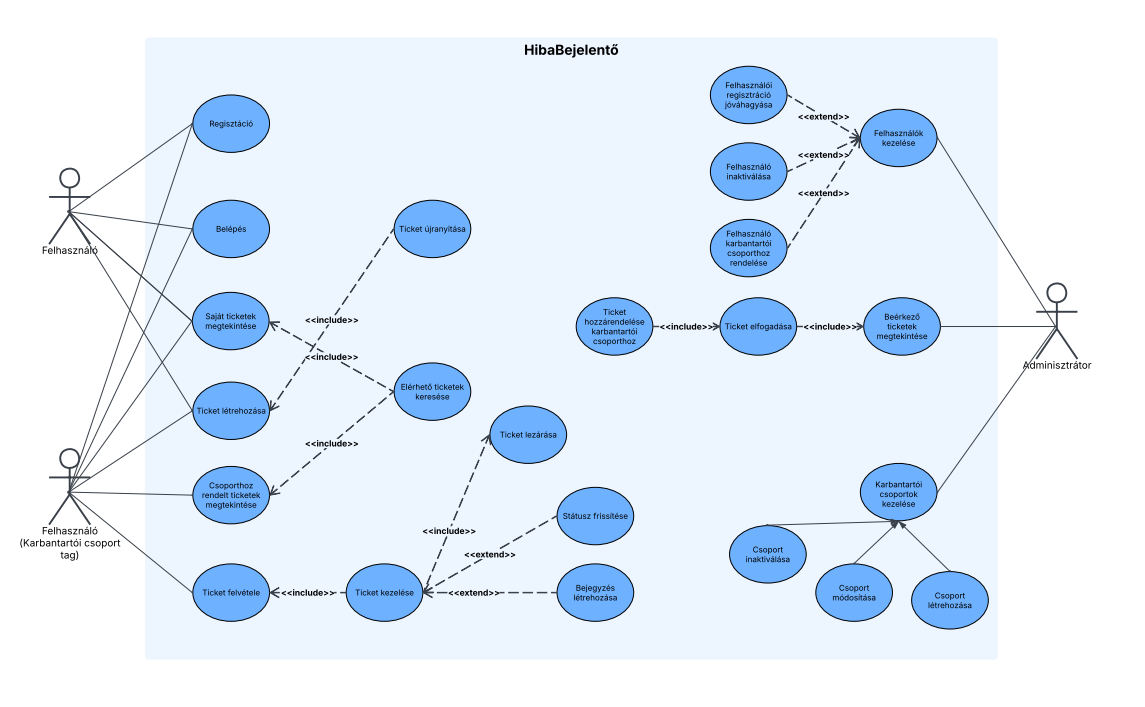
\includegraphics[width=0.98\textwidth,height=0.68\textheight,keepaspectratio]{UseCase.png}}
        {\fbox{\parbox{0.85\textwidth}{\centering
        A Use Case-ábra helye. Töltsd fel a képet UseCase.png néven az Overleaf-projektbe.}}}
    \caption{A hibabejelentő rendszer használatieset-diagramja}
    \label{fig:use-case}
\end{figure}

\subsection{A bejelentő használati esetei}

A bejelentő regisztrációval kezdeményezheti a rendszer használatát. A regisztráció jóváhagyását követően bejelentkezhet, hibabejelentést hozhat létre, és áttekintheti a saját bejelentéseit. A bejelentés egyedi azonosítója alapján visszakeresheti az adott ticketet.

A bejelentő a tickethez kapcsolódó bejegyzésben válaszolhat a karbantartónak, megtekintheti a ticket bejegyzéseit és státuszelőzményeit. A lezárt ticketet indoklással újranyithatja, saját hibajegyét pedig visszavonhatja. Az alkalmazáson belüli értesítések megtekintése tervezett funkció.

\subsection{A karbantartó használati esetei}

A karbantartó a saját bejelentésein túl külön listában láthatja a karbantartói csoportjához rendelt ticketeket. A csoporthoz rendelt, még fel nem vett bejelentést magára veheti, ezzel jelezve, hogy ő végzi a kezelését.

A felvett ticket kezelése során bejegyzést írhat, amely a ticketet automatikusan \textit{Válaszra vár} állapotba helyezi. A munka végén végső bejegyzéssel és lezárási típussal lezárja a bejelentést. A csoporthoz rendelt ticketek bejegyzéseit és státuszelőzményeit akkor is megtekintheti, ha a ticketet a csoport egy másik tagja vette fel.

\subsection{Az adminisztrátor használati esetei}

Az adminisztrátor a regisztrációkat jóváhagyhatja, felhasználókat inaktiválhat és karbantartói csoporthoz rendelhet. Kezeli a csoportokat, a hibakategóriákat, a helyszíneket és a prioritásokat. Az összes hibajegyet áttekintheti, az új hibajegyeket elfogadhatja, és az elfogadáskor beállítja a csoportot, a kategóriát és a prioritást.

Az adminisztrátor bármely ticket státuszelőzményét lekérheti. A bejelentő és a karbantartó közötti bejegyzéseket a jelenlegi megvalósításban adminisztrátori jogon nem éri el, és a ticketek kezelésébe sem avatkozik be.

\subsection{Jogosultsági összefoglaló}

A \ref{tab:permissions}. táblázat a hibajegyekkel kapcsolatos fő műveleteket és az ezekre jogosult szereplőket foglalja össze a backend jelenlegi ellenőrzései alapján. A \textit{Csoporttag} oszlop a ticket csoportjába tartozó, de a ticketet fel nem vevő karbantartót, a \textit{Felvevő} oszlop pedig a ticketet felvevő karbantartót jelöli.

\begin{table}[H]
    \centering
    \footnotesize
    \setstretch{1.15}
    \begin{tabular}{>{\raggedright\arraybackslash}p{5.2cm}cccc}
        \toprule
        \textbf{Művelet} & \textbf{Bejelentő} & \textbf{Csoporttag} & \textbf{Felvevő} & \textbf{Admin} \\
        \midrule
        Hibajegy létrehozása & igen & igen & igen & igen \\
        Saját bejelentések listája & igen & igen & igen & igen \\
        Csoport ticketjeinek listája & -- & igen & igen & -- \\
        Összes ticket listája & -- & -- & -- & igen \\
        Ticket lekérése azonosító alapján & igen & igen & igen & igen \\
        Új ticket elfogadása & -- & -- & -- & igen \\
        Ticket felvétele & -- & igen & -- & -- \\
        Bejegyzések megtekintése & igen & igen & igen & -- \\
        Bejegyzés írása & igen & -- & igen & -- \\
        Lezárás & -- & -- & igen & -- \\
        Újranyitás & igen & -- & -- & -- \\
        Visszavonás & igen & -- & -- & -- \\
        Státuszelőzmény megtekintése & igen & igen & igen & igen \\
        \bottomrule
    \end{tabular}
    \caption{A hibajegyműveletek jogosultságai szerepkörönként}
    \label{tab:permissions}
\end{table}

\section{Választott technológiák}

A rendszer egy asztali kliensből, egy HTTP-alapú alkalmazásprogramozási felületből (API) és egy szerveroldali adatbázisból áll. A kliens feladata a felhasználói felület megjelenítése és a felhasználói műveletek kezdeményezése. Az üzleti szabályok ellenőrzése és az adatok kezelése a Web API feladatkörébe tartozik. Az adatbázist a kliens nem éri el közvetlenül.

\subsection{Frontend}

A kliensalkalmazás .NET MAUI keretrendszerrel, C\# nyelven készül. A MAUI lehetőséget ad arra, hogy a felhasználói felület és az alkalmazás logikájának jelentős része közös projektben készüljön el. A projekt jelenlegi célplatformja a Windows asztali környezet.

A kliens a szerverrel HTTP-kéréseken keresztül kommunikál. Az API elérését szolgáltatásosztály végzi. A kliens bejelentkezéskor megkapja a hozzáférési tokent, amelyet a védett végpontok hívásakor Bearer tokenként küld el.

A kliens nem tárolja és nem kezeli közvetlenül az SQLite-adatbázist. Ez a kialakítás elkülöníti a felhasználói felületet az adatkezeléstől, és lehetővé teszi, hogy az üzleti szabályokat a szerver ellenőrizze.

\subsection{Backend}

A szerveroldali alkalmazás ASP.NET Core Web API formájában készült C\# nyelven, a .NET 10 célkeretrendszerrel. A Web API fogadja a kliens kéréseit, ellenőrzi azok érvényességét és a felhasználói jogosultságokat, végrehajtja az üzleti szabályokat, majd választ küld a kliensnek.

Az adatkezelés Entity Framework Core segítségével, SQLite-adatbázison keresztül történik. Az adatbázis sémaváltozásait Entity Framework Core-migrációk írják le, amelyeket az alkalmazás induláskor automatikusan alkalmaz. A kliens nem fér hozzá közvetlenül az adatbázishoz.

A backend a felhasználói regisztrációt és bejelentkezést, a JWT-alapú hitelesítést, a jogosultság-ellenőrzést, a hibajegyek teljes életciklusának kezelését, a bejegyzéseket és státuszelőzményeket, valamint a csoportok, kategóriák, helyszínek, prioritások, felhasználók és hibajegyek adminisztratív végpontjait tartalmazza.

A fejlesztői környezetben az API OpenAPI-leírást és Swagger felületet biztosít a végpontok áttekintéséhez és Bearer tokennel történő kipróbálásához.

\section{Szoftverarchitektúra}

\subsection{Rendszerfelépítés}

A rendszer három fő részből áll:

\begin{itemize}
    \item \textbf{MAUI kliens:} megjeleníti a felhasználói felületet, összegyűjti a felhasználó által megadott adatokat, és kéréseket küld az API-nak.
    \item \textbf{Web API:} fogadja és feldolgozza a kliens kéréseit, ellenőrzi az üzleti szabályokat, kezeli a jogosultságokat, valamint elvégzi az adatbázis-műveleteket.
    \item \textbf{SQLite-adatbázis:} a szerveroldali alkalmazás által kezelt adatokat tárolja, például a felhasználókat, csoportokat, bejelentéseket, bejegyzéseket és státuszelőzményeket.
\end{itemize}

\begin{figure}[htbp]
    \centering
    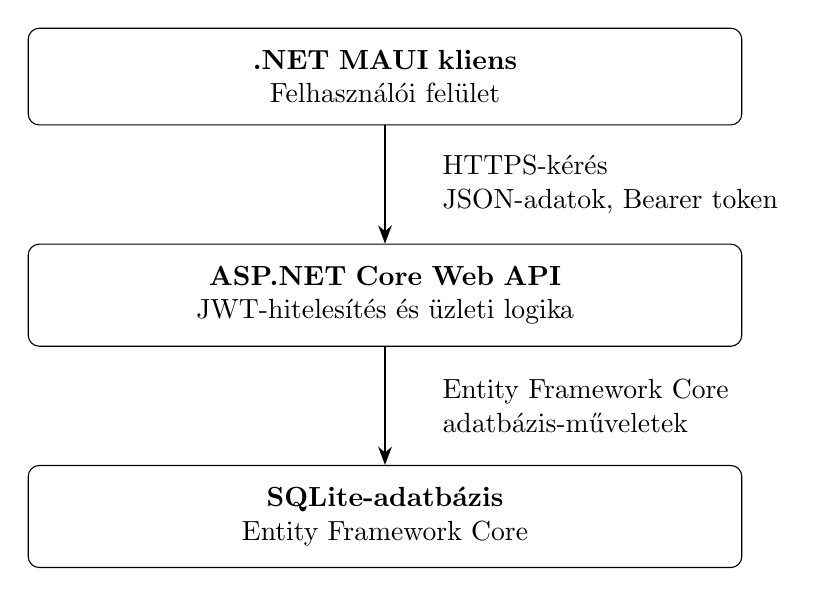
\begin{tikzpicture}[
        node distance=1.5cm,
        box/.style={
            draw,
            rounded corners,
            align=center,
            text width=8.5cm,
            minimum height=1.15cm,
            inner sep=8pt
        },
        arrow/.style={-{Stealth}, thick}
    ]
        \node[box] (client) {
            \textbf{.NET MAUI kliens}\\
            Felhasználói felület
        };

        \node[box, below=of client] (api) {
            \textbf{ASP.NET Core Web API}\\
            JWT-hitelesítés és üzleti logika
        };

        \node[box, below=of api] (database) {
            \textbf{SQLite-adatbázis}\\
            Entity Framework Core
        };

        \draw[arrow] (client.south) -- (api.north)
            node[midway, right=0.6cm, align=left, text width=4.5cm] {
                HTTPS-kérés\\
                JSON-adatok, Bearer token
            };

        \draw[arrow] (api.south) -- (database.north)
            node[midway, right=0.6cm, align=left, text width=4.5cm] {
                Entity Framework Core\\
                adatbázis-műveletek
            };
    \end{tikzpicture}
    \caption{A rendszer komponensei és a közöttük zajló kommunikáció}
    \label{fig:architecture}
\end{figure}

A kliens a Web API-n keresztül kezdeményez adatlekérést vagy adatváltoztatást. A szerver ellenőrzi, hogy a kérés megfelel-e a rendszer szabályainak, majd szükség esetén módosítja az adatbázist. A kliens a szerver válasza alapján frissíti a megjelenített adatokat.

Ez az architektúra a felhasználói felületet, az üzleti logikát és az adattárolást különíti el. Ennek eredményeként az adatbázis közvetlenül nem érhető el a kliensből, az adatokat érintő döntések pedig egy helyen, a szerveren kezelhetők.

\subsection{A backend projekt felépítése}

A Web API projekt mappaszerkezete a felelősségi körök szerint tagolódik:

\begin{itemize}
    \item \texttt{Controllers} -- a HTTP-végpontokat tartalmazó vezérlők. A felhasználói műveletek (\texttt{Auth}, \texttt{Tickets}, \texttt{Categories}, \texttt{Locations}, \texttt{Priorities}, \texttt{Health}) és az adminisztratív műveletek (\texttt{Admin}-előtagú vezérlők) külön osztályokban szerepelnek.
    \item \texttt{DTOs} -- a kérések és válaszok adatátviteli objektumai, a bemenetek validációs attribútumaival.
    \item \texttt{Data} -- az \texttt{AppDbContext} osztály, amely a táblákat, kulcsokat, indexeket, hosszkorlátokat és kapcsolatokat írja le.
    \item \texttt{Middleware/Entities} és \texttt{Middleware/Enums} -- az adatbázis-entitások és a felsorolt típusok (például a ticketállapot és a lezárási típus).
    \item \texttt{Migrations} -- az EF Core által generált migrációk.
    \item \texttt{Services} és \texttt{Options} -- a JWT-token előállítása és a JWT-beállítások.
    \item \texttt{Extensions} -- az OpenAPI-leírás Bearer-sémájának beállítása a Swagger számára.
\end{itemize}

Az üzleti logika jelenleg a vezérlőkben található, a vezérlők közvetlenül az \texttt{AppDbContext} osztályon keresztül érik el az adatbázist. A \texttt{Repositories} mappa a későbbi rétegzéshez előkészített, de még üres. A projekt méretéhez ez a megoldás egyelőre átlátható, a továbbfejlesztés során azonban a közös logika -- például a munkanap-számítás és a válaszobjektum összeállítása -- szolgáltatásosztályba emelhető.

A jogosultság-ellenőrzés két szinten történik. A vezérlőkön lévő \texttt{[Authorize]} attribútum biztosítja, hogy csak érvényes tokennel lehessen a végpontokat hívni. Ezen felül minden művelet az adatbázisból olvassa ki a felhasználó aktuális adatait -- aktív-e, jóváhagyott-e, adminisztrátor-e, melyik csoport tagja --, és ezek alapján dönt. Így egy csoportváltás vagy inaktiválás azonnal érvényesül, nem kell megvárni a token lejártát.

\subsection{Adatbázis kialakítása}

A rendszer adatbázisa a Web API által kezelt SQLite-adatbázis. Az adatmodell relációs felépítésű: a bejelentések a felhasználókhoz, csoportokhoz, kategóriákhoz, helyszínekhez és prioritásokhoz kapcsolódnak. A ticketek bejegyzéseit és állapotelőzményeit külön táblák tárolják.

\begin{figure}[htbp]
    \centering
    \IfFileExists{AdatbazisTerv.png}
        {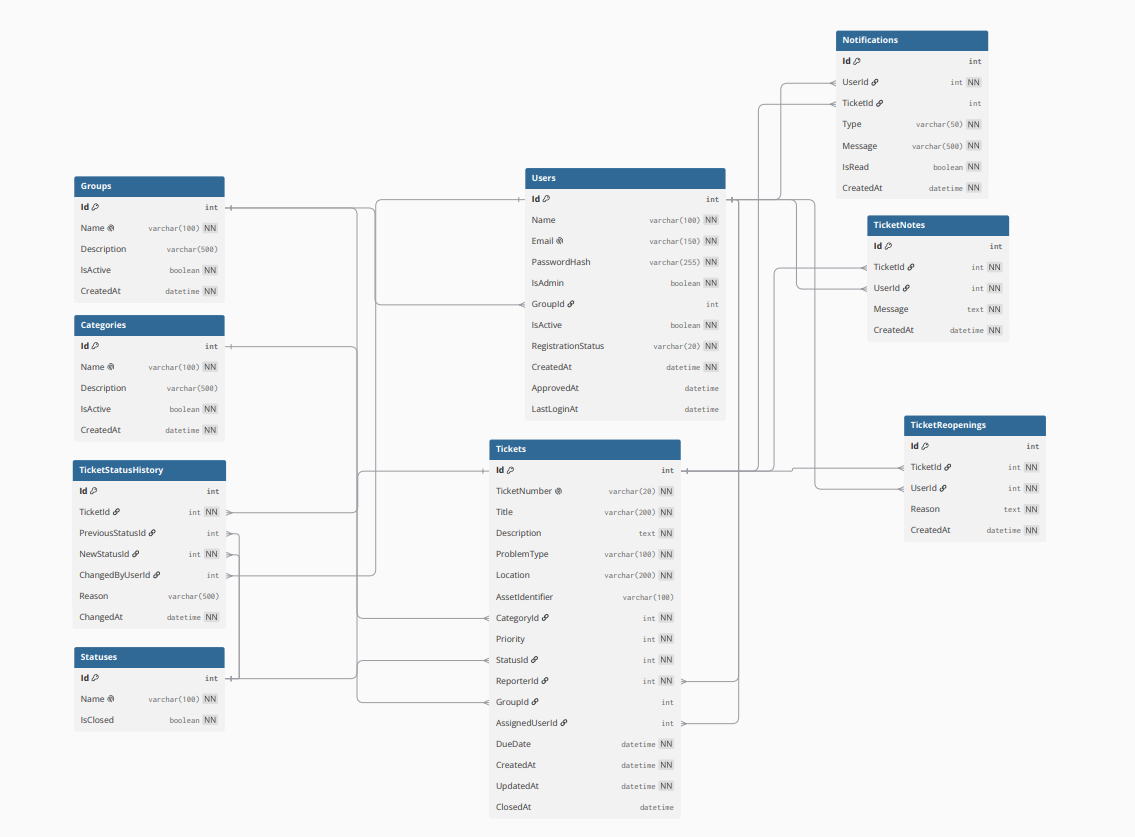
\includegraphics[width=0.98\textwidth,height=0.68\textheight,keepaspectratio]{AdatbazisTerv.png}}
        {\fbox{\parbox{0.85\textwidth}{\centering
        Az adatbázisterv ábrájának helye. Töltsd fel a képet AdatbazisTerv.png néven az Overleaf-projektbe.}}}
    \caption{A hibabejelentő rendszer adatmodellje}
    \label{fig:database}
\end{figure}

\subsubsection{Felhasználók és karbantartói csoportok}

A \texttt{Users} tábla tárolja a felhasználó nevét, e-mail-címét, jelszóhash-ét, aktív állapotát és regisztrációs állapotát, valamint a regisztráció, a jóváhagyás és az utolsó bejelentkezés időpontját. Az e-mail-cím egyedi. Az adminisztrátori jogosultságot az \texttt{IsAdmin} mező jelzi.

A karbantartói csoporttagságot a felhasználó \texttt{GroupId} mezője rögzíti. Egy csoporthoz több felhasználó tartozhat, egy felhasználó viszont legfeljebb egy csoport tagja lehet. A \texttt{Groups} tábla a csoport egyedi nevét, leírását és aktív állapotát tárolja. A csoportokat az adminisztrátor kezeli.

A felhasználók törlése helyett az inaktiválás használható. Ez megőrzi a korábbi bejelentésekhez, bejegyzésekhez és státuszelőzményekhez fűződő kapcsolatokat.

\subsubsection{Bejelentések, kategóriák és helyszínek}

A \texttt{Tickets} tábla tartalmazza a bejelentés egyedi azonosítóját, címét, leírását, helyszínét és opcionális eszközazonosítóját. Emellett rögzíti a bejelentőt, a kategóriát, a prioritást, az aktuális állapotot, a hozzárendelt csoportot, a ticketet felvevő karbantartót, a határidőt és az időadatokat.

A \texttt{TicketNumber} mező egyedi, felhasználók számára megjeleníthető azonosítót tárol \texttt{HIB-ÉÉÉÉHHNN-XXXXXXXX} formában, például \texttt{HIB-20261109-A52010C3}. A dátumrész a létrehozás napját, az utolsó nyolc karakter egy véletlenszerűen generált GUID nagybetűs elejét tartalmazza. A \texttt{ReporterId} jelöli a bejelentőt, a \texttt{GroupId} az illetékes karbantartói csoportot, az \texttt{AssignedUserId} pedig a ticketet felvevő karbantartót. Az utóbbi két mező addig üres, amíg az adminisztrátor el nem fogadja a ticketet, illetve amíg egy karbantartó fel nem veszi.

A helyszín a \texttt{LocationId} idegen kulccsal kapcsolódik a \texttt{Locations} táblához. A ticket ezen felül a létrehozáskori helyszínnevet szövegként is eltárolja a \texttt{Location} mezőben. Ez megjelenítési pillanatkép: egy helyszín későbbi átnevezése nem írja át a korábbi ticketeken látható nevet. Az \texttt{AssetIdentifier} opcionális, legfeljebb 100 karakteres mező.

A \texttt{Categories} és a \texttt{Locations} tábla az adminisztrátor által kezelt kategóriákat és helyszíneket tartalmazza. Mindkét táblában a név egyedi, és mindkettőhöz tartozik leírás és aktív állapot. A már használt kategóriát és helyszínt inaktiválni lehet, törölni nem, így a korábbi bejelentések hivatkozásai megmaradnak. Új ticket csak aktív kategóriával és aktív helyszínnel hozható létre.

\subsubsection{Prioritás és határidő}

A prioritásokat a \texttt{Priorities} tábla tárolja. Minden prioritásnak egyedi neve (2--20 karakter), munkanapban megadott határidője (\texttt{DefaultDueDays}, 1--365), alapértelmezettséget jelző mezője (\texttt{IsDefault}) és aktív állapota van. A ticket a \texttt{PriorityId} idegen kulccsal kapcsolódik a prioritáshoz, és a helyszínhez hasonlóan a prioritás nevét is eltárolja pillanatképként.

A prioritások kezelésére az alábbi szabályok vonatkoznak:

\begin{itemize}
    \item mindig pontosan egy aktív alapértelmezett prioritás van; egy új alapértelmezett prioritás kijelölése a korábbitól elveszi ezt a jelölést;
    \item az első létrehozott prioritás kötelezően alapértelmezett;
    \item az alapértelmezett prioritás nem inaktiválható, és nem vehető el róla a jelölés, ha nincs másik aktív alapértelmezett prioritás;
    \item inaktív prioritás nem lehet alapértelmezett;
    \item a határidő módosítása csak az ezt követően létrehozott vagy elfogadott ticketekre hat, a meglévő ticketek határideje nem számolódik újra.
\end{itemize}

A kezdeti adatbázisban szereplő értékek:

\begin{itemize}
    \item Sürgős: 1 munkanap;
    \item Magas: 3 munkanap;
    \item Normál: 5 munkanap (alapértelmezett);
    \item Alacsony: 10 munkanap.
\end{itemize}

A határidő számításakor a hétfőtől péntekig tartó napok számítanak munkanapnak. A jelenlegi megvalósítás nem használ külön munkaszüneti-naptárat. A ticket létrehozásakor az alapértelmezett prioritáshoz tartozó határidő kerül kiszámításra. Adminisztrátori elfogadáskor a kiválasztott prioritás alapján, az elfogadás időpontjától számítva a határidő újraszámolódik.

A korábbi változatban a prioritás C\# enumként szerepelt. A helyszínek és prioritások adminisztrálhatóvá tételekor egy migráció a meglévő ticketek szöveges helyszínértékeiből létrehozta a \texttt{Locations} rekordokat, a szöveges prioritásértékeket pedig az új \texttt{Priorities} rekordokhoz rendelte. Így a korábban létrehozott ticketek adatai az átállás után is megmaradtak.

\subsubsection{Bejegyzések}

A \texttt{TicketNotes} tábla tárolja a ticketekhez írt bejegyzéseket. Egy rekord tartalmazza a ticket és a szerző azonosítóját, a legfeljebb 5000 karakteres üzenetet, a létrehozás időpontját, valamint az opcionális \texttt{ClosureTypeId} mezőt. Ez utóbbi csak a lezáráskor létrehozott végső bejegyzésnél van kitöltve, és a lezárási típus számát (1--5) tárolja. A ticket újranyitásakor az indoklás szintén bejegyzésként kerül rögzítésre.

A bejegyzésekhez nincs módosító vagy törlő végpont, és az idegen kulcsok korlátozó törlési szabályt használnak. A bejegyzések így a ticket teljes kommunikációs előzményét változatlan formában őrzik meg. A tábla a ticketazonosító és a létrehozási idő együttesére indexet tartalmaz, mivel a bejegyzések lekérése mindig e két mező szerint történik.

\subsubsection{Állapotok és állapotváltozási előzmények}

A backend a hibajegyekhez az alábbi állapotokat használja: \texttt{Új}, \texttt{Folyamatban}, \texttt{VálaszraVár}, \texttt{Lezárt}, \texttt{Újranyitva} és \texttt{Visszavonva}. Az állapot az adatbázisban szövegként tárolódik, és az API JSON-válaszaiban is szöveges értékként jelenik meg.

A ticket aktuális állapotát az adatbázis a \texttt{Tickets} rekord részeként tárolja. A \texttt{TicketStatusHistory} tábla minden állapotváltozást rögzít: a létrehozást, az adminisztrátori elfogadást, a bejegyzések által kiváltott automatikus változásokat, a lezárást, az újranyitást és a visszavonást. Ha egy esemény nem változtat az állapoton -- például a karbantartói felvétel vagy egy \textit{Folyamatban} állapotú ticketen írt bejelentői bejegyzés --, nem keletkezik előzményrekord.

Az előzményrekord tartalmazza a ticket azonosítóját, az előző és az új állapotot, a változás időpontját, a változást kiváltó felhasználót és a változás indokát. Az első rekordban az előző állapot üres. Lezáráskor az indok a lezárási típust, újranyitáskor a bejelentő indoklását tartalmazza.

\subsubsection{A fő táblák és kapcsolataik összefoglalása}

\begin{itemize}
    \item Egy csoporthoz több felhasználó tartozhat; egy felhasználó legfeljebb egy csoporthoz rendelhető.
    \item Egy felhasználó több bejelentést hozhat létre, és több ticketet vehet fel karbantartóként.
    \item Egy csoport több bejelentést kaphat.
    \item Egy kategóriához, helyszínhez és prioritáshoz több bejelentés tartozhat.
    \item Egy tickethez több bejegyzés és több állapotváltozási előzmény tartozhat.
\end{itemize}

\begin{table}[H]
    \centering
    \footnotesize
    \setstretch{1.15}
    \begin{tabular}{>{\raggedright\arraybackslash}p{3.2cm}>{\raggedright\arraybackslash}p{11.5cm}}
        \toprule
        \textbf{Tábla} & \textbf{Fontosabb mezők} \\
        \midrule
        \texttt{Users} & Id, Name, Email (egyedi), PasswordHash, IsAdmin, GroupId, IsActive, RegistrationStatus, CreatedAt, ApprovedAt, LastLoginAt \\
        \texttt{Groups} & Id, Name (egyedi), Description, IsActive, CreatedAt \\
        \texttt{Categories} & Id, Name (egyedi), Description, IsActive, CreatedAt \\
        \texttt{Locations} & Id, Name (egyedi), Description, IsActive, CreatedAt \\
        \texttt{Priorities} & Id, Name (egyedi), DefaultDueDays, IsDefault, IsActive, CreatedAt \\
        \texttt{Tickets} & Id, TicketNumber (egyedi), Title, Description, LocationId, Location, AssetIdentifier, CategoryId, PriorityId, Priority, Status, ReporterId, GroupId, AssignedUserId, DueDate, IsActive, CreatedAt, UpdatedAt, ClosedAt \\
        \texttt{TicketNotes} & Id, TicketId, UserId, Message, ClosureTypeId, CreatedAt \\
        \texttt{TicketStatusHistory} & Id, TicketId, OldStatus, NewStatus, ChangedByUserId, Reason, CreatedAt \\
        \bottomrule
    \end{tabular}
    \caption{Az adatbázis táblái és fontosabb mezői}
    \label{tab:tables}
\end{table}

A kapcsolatok alapján az adatbázis megőrzi, ki hozta létre a bejelentést, melyik csoport felelős érte, ki kezelte, milyen kommunikáció zajlott, és hogyan változott az állapota. Minden idegen kulcs korlátozó törlési szabályt használ, így olyan rekord, amelyre más rekord hivatkozik, nem törölhető véletlenül.

\subsection{Asztali alkalmazás}

Az asztali alkalmazás a felhasználói szerepköröknek megfelelő funkciókat jelenít meg. A bejelentői, karbantartói és adminisztrátori felületek eltérő műveleteket tesznek elérhetővé, miközben ugyanahhoz a Web API-hoz kapcsolódnak.

A kliensben jelenleg a bejelentői folyamat alapjai készültek el: a bejelentkezés, a hibajegylista keresése és szűrése, a hibajegy adatainak megjelenítése és új hibajegy létrehozása. A karbantartói és adminisztrátori munkafolyamat backendoldalon már elérhető, ezek felülete a következő fejlesztési szakasz feladata.

\subsubsection{Bejelentkezés}

Az alkalmazás indulásakor a bejelentkező képernyő jelenik meg. A felhasználó e-mail-címet és jelszót ad meg, a kliens pedig a \texttt{POST /api/auth/login} végpontot hívja. Siker esetén a kliens eltárolja a kapott hozzáférési tokent, és a további kérésekhez Bearer tokenként használja. Jóváhagyásra váró, inaktív vagy hibás adatokkal rendelkező fiók esetén a backend egységes hibaüzenetet ad, így nem derül ki, hogy a megadott e-mail-cím létezik-e.

\begin{figure}[H]
    \centering
    \IfFileExists{Login.png}
        {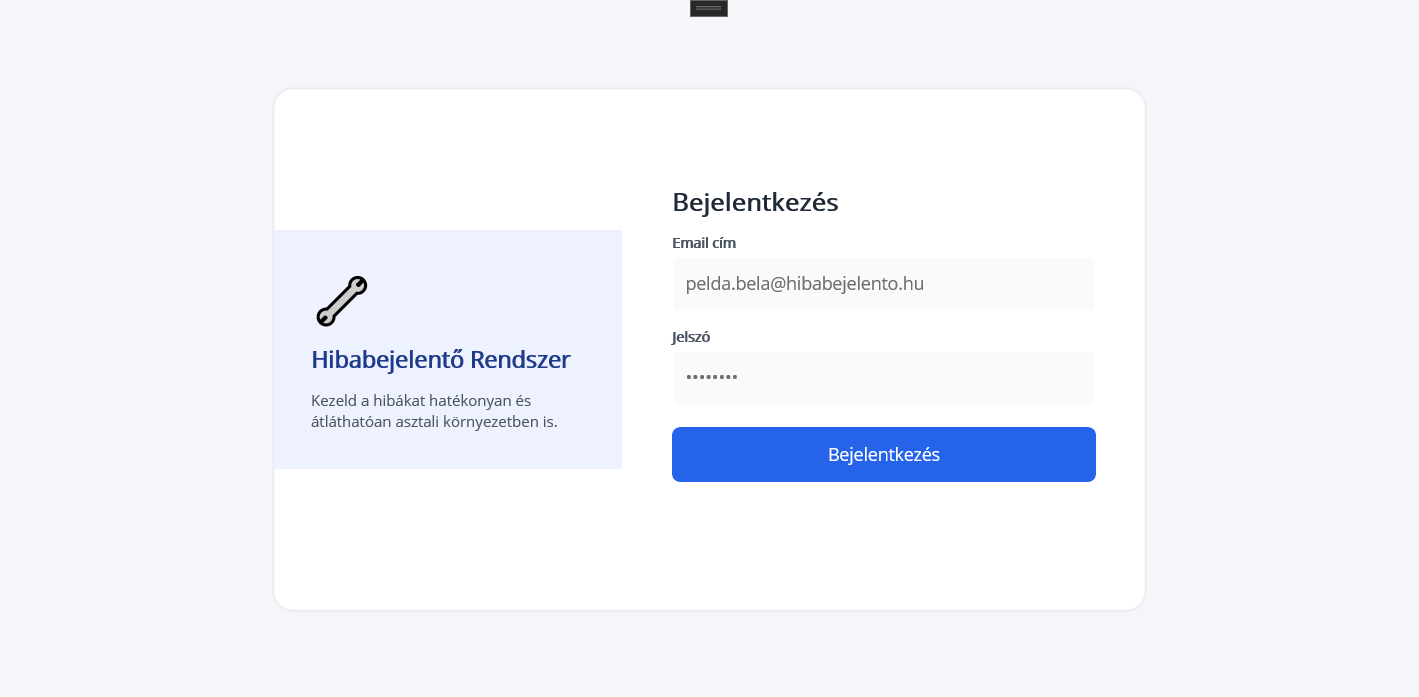
\includegraphics[width=0.95\textwidth,height=0.34\textheight,keepaspectratio]{Login.png}}
        {}
    \caption{A kliens bejelentkező képernyője}
    \label{fig:gui-login}
\end{figure}

\subsubsection{Hibajegylista, keresés és szűrés}

Bejelentkezés után a felhasználó a hibajegyeinek listáját látja. A táblázat oszlopai: azonosító, megnevezés, prioritás, státusz, bejelentő és határidő. A lista feletti keresőmező a hibajegyek közötti szöveges keresést, a mellette lévő legördülő mező az állapot szerinti szűrést teszi lehetővé, az \textit{Összes} érték esetén minden ticket látszik. A képernyőről érhető el a kijelentkezés és az új hibajegy létrehozása (\textit{+ Új}) is.

A lista adatai a backend listázó végpontjából származnak. A keresés és a szűrés a már lekért listán belül történik, a szerveroldali, bővített keresés továbbfejlesztési feladat.

\begin{figure}[H]
    \centering
    \IfFileExists{TicketLista.png}
        {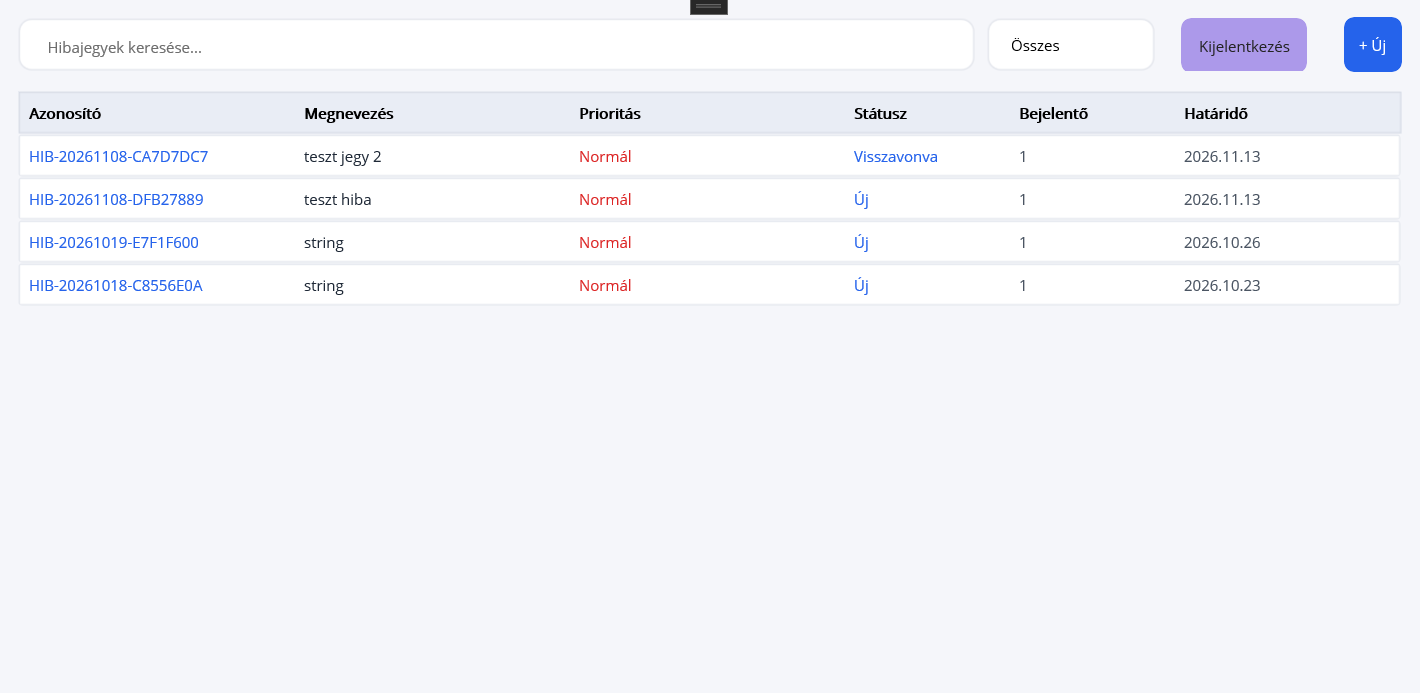
\includegraphics[width=0.95\textwidth,height=0.34\textheight,keepaspectratio]{TicketLista.png}}
        {}
    \caption{A hibajegylista kereséssel és állapotszűrővel}
    \label{fig:gui-list}
\end{figure}

\subsubsection{Új hibajegy létrehozása}

Az új hibajegy űrlapján a felhasználó megadja a hibajegy címét, kategóriáját, helyszínét, opcionálisan az érintett eszköz azonosítóját, valamint a hiba leírását. A kötelező mezőket csillag jelöli. A kategóriák az aktív kategóriák végpontjáról töltődnek be. A \textit{Ticket létrehozása} gomb a \texttt{POST /api/tickets} végpontot hívja; a backend validálja a mezőket, kiosztja az egyedi azonosítót, beállítja az alapértelmezett prioritást és a határidőt.

\begin{figure}[H]
    \centering
    \IfFileExists{TicketAdd.png}
        {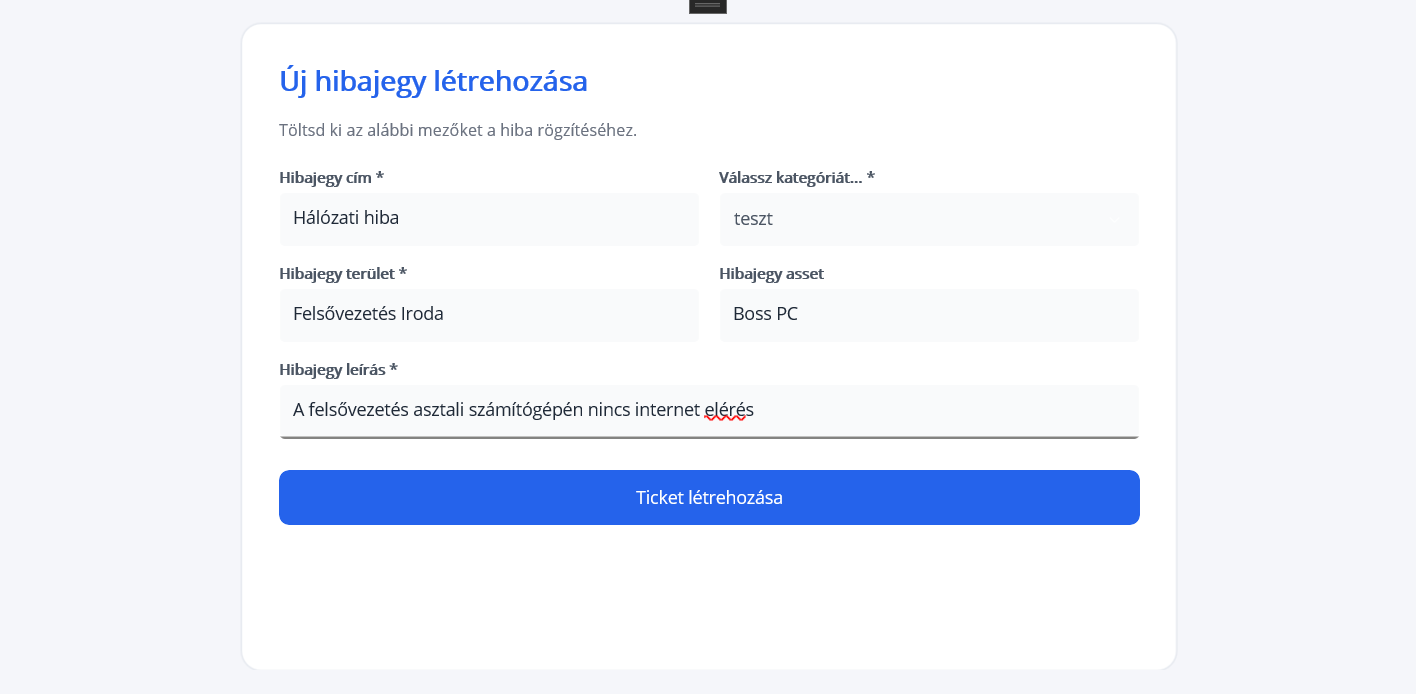
\includegraphics[width=0.95\textwidth,height=0.34\textheight,keepaspectratio]{TicketAdd.png}}
        {}
    \caption{Új hibajegy létrehozása}
    \label{fig:gui-add}
\end{figure}

\subsubsection{Hibajegy adatainak megjelenítése}

A listában egy azonosítóra kattintva megnyílik a hibajegy részletes nézete. Bal oldalon az azonosító, a státusz, a prioritás, a kategória, a bejelentő és a határidő látható, jobb oldalon a leírás, az eszközazonosító és a helyszín. Az eseménynapló a ticket életciklusának eseményeit időrendben jeleníti meg. A nézet alján található \textit{Hibajegy visszavonása} gomb a \texttt{POST /api/tickets/\{id\}/withdraw} végpontot hívja.

\begin{figure}[H]
    \centering
    \IfFileExists{TicketDetail.png}
        {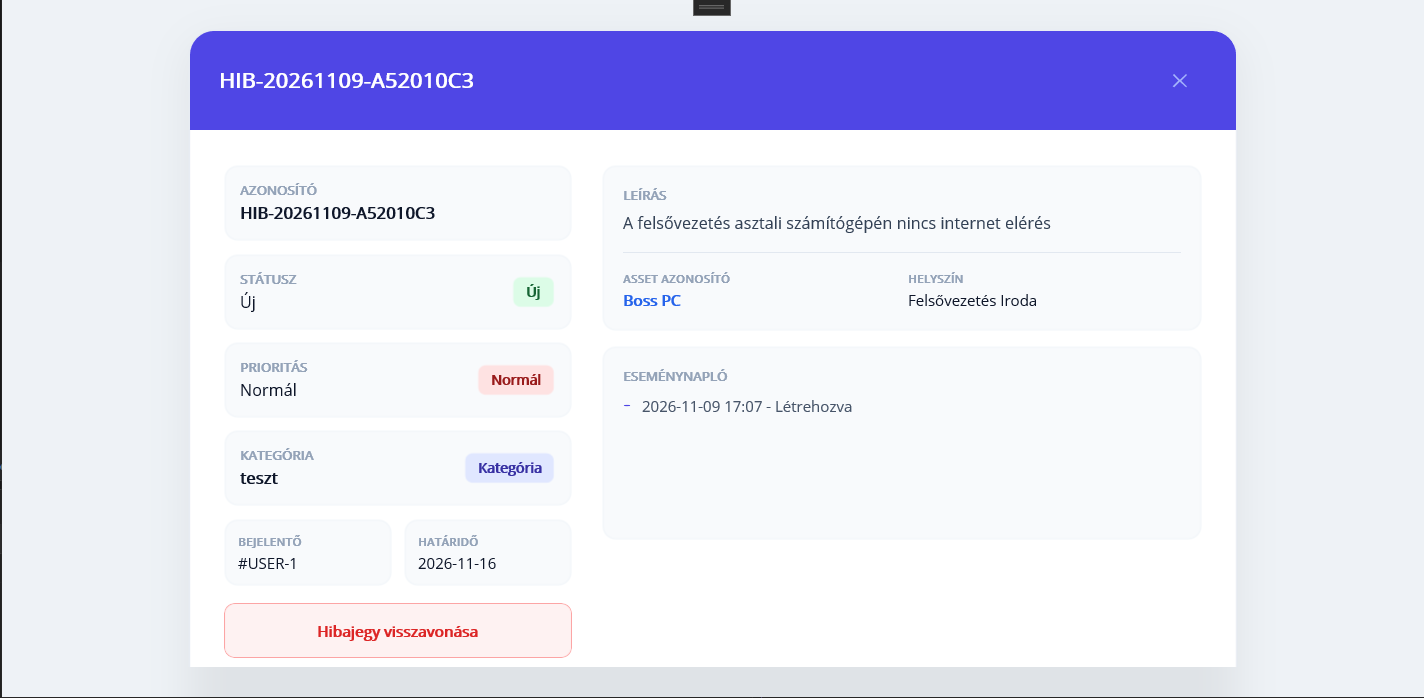
\includegraphics[width=0.95\textwidth,height=0.34\textheight,keepaspectratio]{TicketDetail.png}}
        {}
    \caption{A hibajegy részletes adatai és eseménynaplója}
    \label{fig:gui-detail}
\end{figure}

A bejelentő mezőben jelenleg a felhasználó azonosítója jelenik meg, mivel a ticket válaszobjektuma a bejelentőnek csak az azonosítóját tartalmazza, a nevét nem. A felvevő karbantartó nevét a válasz már tartalmazza, a bejelentő nevének hozzáadása kisebb backendmódosítással megoldható.

\section{Kommunikációs rendszer kialakítása (API)}

\subsection{Az API szerepe}

A MAUI-kliens és a szerveroldali alkalmazás HTTP-alapú API-n, JSON-formátumú kérésekkel és válaszokkal kommunikál. A kliens a Web API-n keresztül kér adatot vagy kezdeményez módosítást; az adatbázishoz közvetlenül nem kapcsolódik.

A backend felel a bemenetek ellenőrzéséért, a hitelesítésért, a jogosultságok vizsgálatáért és az adatbázis-műveletek végrehajtásáért. A \texttt{GET /api/health} kivételével minden végpont csak Bearer tokennel érhető el.

A \texttt{GET /api/health} végpont az API és az adatbázis kapcsolatának állapotáról ad visszajelzést. A fejlesztői környezetben az OpenAPI-dokumentáció a Swagger felületen keresztül érhető el.

\subsection{Megvalósított API-végpontok}

A \ref{tab:endpoints}. táblázat a backendben megvalósított HTTP-végpontokat foglalja össze. Az \texttt{\{id\}} egész számú adatbázis-azonosítót, a \texttt{\{ticketNumber\}} pedig egy egyedi hibajegyazonosítót jelöl. A \textit{Jogosult} oszlopban a \textit{Belépett} bármely aktív, jóváhagyott felhasználót jelent.

{\footnotesize
\setstretch{1.1}
\begin{longtable}{>{\raggedright\arraybackslash}p{1.1cm}>{\raggedright\arraybackslash}p{6.9cm}>{\raggedright\arraybackslash}p{2.3cm}>{\raggedright\arraybackslash}p{4.3cm}}
    \caption{A backend HTTP-végpontjai}
    \label{tab:endpoints}\\
    \toprule
    \textbf{Metódus} & \textbf{Útvonal} & \textbf{Jogosult} & \textbf{Leírás} \\
    \midrule
    \endfirsthead
    \toprule
    \textbf{Metódus} & \textbf{Útvonal} & \textbf{Jogosult} & \textbf{Leírás} \\
    \midrule
    \endhead
    \bottomrule
    \endfoot
    \multicolumn{4}{l}{\textbf{Általános és hitelesítés}} \\
    GET & \texttt{/api/health} & bárki & API és adatbázis állapota \\
    POST & \texttt{/api/auth/register} & bárki & regisztráció, jóváhagyásra vár \\
    POST & \texttt{/api/auth/login} & bárki & bejelentkezés, JWT kiadása \\
    GET & \texttt{/api/auth/me} & Belépett & saját felhasználói adatok \\
    \midrule
    \multicolumn{4}{l}{\textbf{Törzsadatok olvasása}} \\
    GET & \texttt{/api/categories} & Belépett & aktív kategóriák \\
    GET & \texttt{/api/locations} & Belépett & aktív helyszínek \\
    GET & \texttt{/api/priorities} & Belépett & aktív prioritások \\
    \midrule
    \multicolumn{4}{l}{\textbf{Hibajegyek}} \\
    POST & \texttt{/api/tickets} & Belépett & új hibajegy létrehozása \\
    GET & \texttt{/api/tickets/mine} & Belépett & saját bejelentések listája \\
    GET & \texttt{/api/tickets/maintenance} & csoporttag & a csoport ticketjeinek listája \\
    GET & \texttt{/api/tickets/\{ticketNumber\}} & bejelentő, csoporttag, admin & ticket lekérése azonosító alapján \\
    POST & \texttt{/api/tickets/\{id\}/take} & csoporttag & ticket felvétele \\
    GET & \texttt{/api/tickets/\{id\}/notes} & bejelentő, csoporttag & bejegyzések lekérése \\
    POST & \texttt{/api/tickets/\{id\}/notes} & bejelentő, felvevő & új bejegyzés \\
    POST & \texttt{/api/tickets/\{id\}/close} & felvevő & lezárás típussal \\
    POST & \texttt{/api/tickets/\{id\}/reopen} & bejelentő & újranyitás indoklással \\
    POST & \texttt{/api/tickets/\{id\}/withdraw} & bejelentő & visszavonás \\
    GET & \texttt{/api/tickets/\{id\}/status-history} & bejelentő, csoporttag, admin & státuszelőzmények \\
    \midrule
    \multicolumn{4}{l}{\textbf{Adminisztráció}} \\
    GET & \texttt{/api/admin/users} & admin & felhasználók listája \\
    POST & \texttt{/api/admin/users/\{id\}/approve} & admin & regisztráció jóváhagyása \\
    PATCH & \texttt{/api/admin/users/\{id\}/deactivate} & admin & felhasználó inaktiválása \\
    PUT & \texttt{/api/admin/users/\{id\}/group} & admin & csoporthoz rendelés vagy eltávolítás \\
    GET & \texttt{/api/admin/groups} & admin & csoportok listája \\
    POST & \texttt{/api/admin/groups} & admin & csoport létrehozása \\
    PUT & \texttt{/api/admin/groups/\{id\}} & admin & csoport módosítása \\
    PATCH & \texttt{/api/admin/groups/\{id\}/deactivate} & admin & csoport inaktiválása \\
    GET & \texttt{/api/admin/categories} & admin & összes kategória \\
    POST & \texttt{/api/admin/categories} & admin & kategória létrehozása \\
    PATCH & \texttt{/api/admin/categories/\{id\}/deactivate} & admin & kategória inaktiválása \\
    GET & \texttt{/api/admin/locations} & admin & összes helyszín \\
    POST & \texttt{/api/admin/locations} & admin & helyszín létrehozása \\
    PUT & \texttt{/api/admin/locations/\{id\}} & admin & helyszín módosítása \\
    PATCH & \texttt{/api/admin/locations/\{id\}/deactivate} & admin & helyszín inaktiválása \\
    GET & \texttt{/api/admin/priorities} & admin & összes prioritás \\
    POST & \texttt{/api/admin/priorities} & admin & prioritás létrehozása \\
    PUT & \texttt{/api/admin/priorities/\{id\}} & admin & név, határidő, alapértelmezettség módosítása \\
    PATCH & \texttt{/api/admin/priorities/\{id\}/deactivate} & admin & prioritás inaktiválása \\
    GET & \texttt{/api/admin/tickets?newOnly=} & admin & összes vagy csak új ticket \\
    POST & \texttt{/api/admin/tickets/\{id\}/accept} & admin & elfogadás, csoport, kategória és prioritás beállítása \\
\end{longtable}
}

A korábbi általános \texttt{GET /api/tickets} listázó végpont helyére két külön végpont került. A \texttt{/mine} kizárólag a felhasználó saját bejelentéseit adja vissza, a \texttt{/maintenance} pedig a felhasználó csoportjához rendelt ticketeket. Ha a felhasználó nem tagja aktív csoportnak, ez utóbbi \texttt{403 Forbidden} választ ad. A szétválasztás miatt a kliens külön nézetben jelenítheti meg a bejelentői és a karbantartói munkát.

Az inaktivált törzsadatok újraaktiválására jelenleg nincs külön végpont; erre szükség esetén a későbbi adminisztrátori felülettel együtt kerülhet sor.

\subsection{Kérések és válaszok}

Az API JSON-formátumú adatokat fogad és ad vissza. A felsorolt típusok, például a ticket állapota, szöveges értékként szerepelnek a JSON-ban. Az időpontok UTC szerint tárolódnak és kerülnek visszaküldésre; a helyi időre alakítás a kliens feladata.

Új hibajegy létrehozásakor a kérés címet, leírást, helyszínazonosítót, kategóriaazonosítót és opcionális eszközazonosítót tartalmaz:

\begin{verbatim}
POST /api/tickets
{
  "title": "Hálózati hiba",
  "description": "A felsővezetés asztali gépén nincs internet.",
  "locationId": 3,
  "categoryId": 1,
  "assetIdentifier": "Boss PC"
}
\end{verbatim}

A cím 3--200 karakter, a leírás legalább 10 karakter lehet, a helyszínnek és a kategóriának léteznie kell és aktívnak kell lennie. Ha nincs aktív alapértelmezett prioritás, a létrehozás \texttt{409 Conflict} választ ad. Sikeres létrehozáskor az API \texttt{201 Created} választ ad, és visszaküldi a létrehozott hibajegy adatait, köztük annak egyedi azonosítóját.

A ticket válaszobjektuma a hibajegy adatain túl a kategória, a csoport és a felvevő karbantartó nevét is tartalmazza, így a kliensnek ezeket nem kell külön lekérnie. A listázó végpontok \texttt{200 OK} választ és a létrehozási idő szerint csökkenő sorrendű JSON-tömböt adnak vissza.

Az adminisztratív elfogadás kérése a célcsoport, a kategória és a prioritás azonosítóját tartalmazza (\texttt{groupId}, \texttt{categoryId}, \texttt{priorityId}). A művelet csak aktív, \textit{Új} állapotú hibajegyen hajtható végre; a backend ellenőrzi a célcsoport, a kategória és a prioritás meglétét, valamint aktivitását. Siker esetén \texttt{204 No Content} a válasz.

A bejegyzés létrehozásának kérése egyetlen \texttt{message} mezőt, a lezárás kérése a lezárási típust (\texttt{closureTypeId}, 1--5) és a végső bejegyzést (\texttt{resolution}) tartalmazza. 
Az újranyitás kérése a \texttt{reason} mezőben az indoklást tartalmazza. A felvétel és a visszavonás kérése nem tartalmaz törzset. A felvétel a frissített ticketet, a lezárás és az újranyitás az új állapotot adja vissza \texttt{200 OK} válasszal, a bejegyzés létrehozása \texttt{201 Created}, a visszavonás \texttt{204 No Content} választ eredményez. A visszavonás ismételt meghívása is \texttt{204} választ ad, így a művelet többszöri végrehajtása nem okoz hibát.

A backend validációs hibánál \texttt{400 Bad Request}, hiányzó vagy érvénytelen hitelesítésnél \texttt{401 Unauthorized}, elégtelen jogosultságnál \texttt{403 Forbidden}, nem létező erőforrásnál \texttt{404 Not Found}, ütköző állapotú műveletnél pedig \texttt{409 Conflict} választ adhat. Ha egy felhasználó olyan ticket bejegyzéseit vagy előzményeit kéri le, amelyhez nincs köze, a backend \texttt{404} választ ad, így a válaszból nem derül ki, hogy a ticket létezik-e.

\subsection{Hitelesítés és jogosultság-ellenőrzés}

A backend JWT Bearer-alapú hitelesítést használ. A regisztráció során létrejövő fiók kezdetben jóváhagyásra vár, ezért az új felhasználó csak adminisztrátori jóváhagyás után jelentkezhet be. A jelszavakat a backend az ASP.NET Core jelszóhash-elő szolgáltatásával hash-elve tárolja; olvasható jelszót nem ment az adatbázisba.

Sikeres bejelentkezéskor az API aláírt JWT hozzáférési tokent állít elő. A token kibocsátója \texttt{Hibabejelento.Api}, célközönsége \texttt{Hibabejelento.Client}, aláírási algoritmusa HMAC-SHA256, érvényességi ideje pedig alapértelmezetten 30 perc. A token a felhasználó azonosítóját, e-mail-címét és nevét tartalmazza; jogosultsági adatot szándékosan nem. A kibocsátó, a célközönség, az aláírókulcs és az érvényességi idő konfigurációból származik; a titkos aláírókulcsot fejlesztés közben User Secrets szolgáltatásban kell tárolni. Ha a beállítások hiányoznak, vagy a kulcs rövidebb 32 bájtnál, az alkalmazás nem indul el.

A kliens a védett végpontokhoz a tokent az alábbi HTTP-fejlécben küldi:

\begin{center}
\texttt{Authorization: Bearer <token>}
\end{center}

A backend ellenőrzi a token aláírását, kibocsátóját, célközönségét és lejárati idejét. A token érvényesítése után az adatbázisban azt is ellenőrzi, hogy a tokenhez tartozó felhasználó továbbra is aktív és jóváhagyott-e; ha nem, a kérést elutasítja. A jogosultsági döntések az adatbázisban tárolt felhasználói adatok alapján történnek; a kliensoldali felület elrejtése önmagában nem jogosultsági ellenőrzés.

Az adminisztratív végpontok külön ellenőrzik, hogy a bejelentkezett és aktív felhasználó adminisztrátori jogosultsággal rendelkezik-e. A hibajegyműveleteknél a backend azt vizsgálja, hogy a felhasználó a ticket bejelentője, felvevője, illetve a ticket csoportjának tagja-e (\ref{tab:permissions}. táblázat).

A rendszer nem használ refresh tokent. Lejárt hozzáférési token esetén a felhasználónak újra be kell jelentkeznie. A token kliensoldali tárolásának és törlésének felelőssége a MAUI-alkalmazásé.

\begin{figure}[htbp]
    \centering
    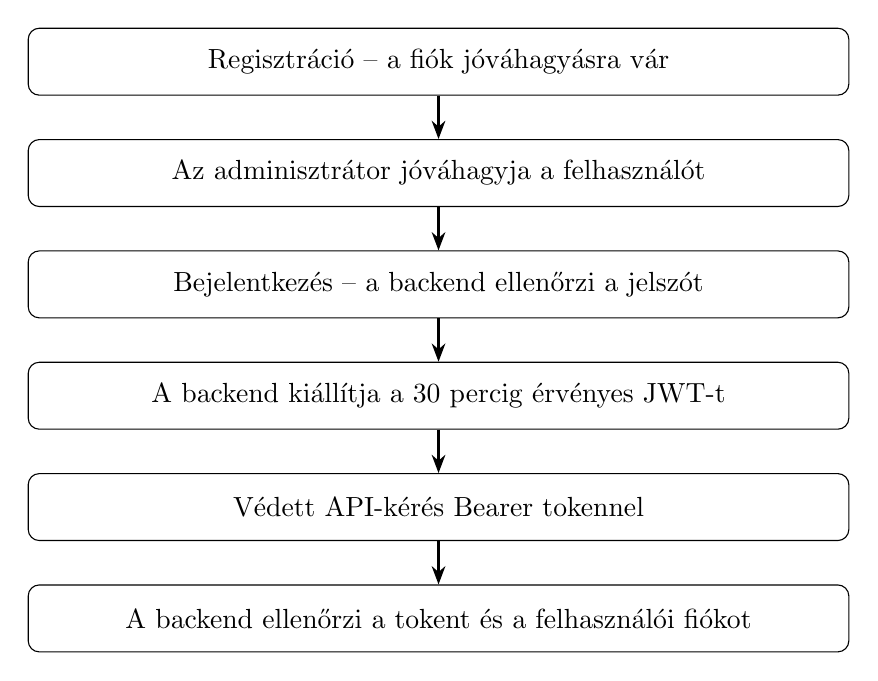
\begin{tikzpicture}[
        node distance=0.55cm,
        flowstep/.style={
            draw,
            rounded corners,
            align=center,
            text width=10cm,
            minimum height=0.85cm,
            inner sep=6pt
        },
        arrow/.style={-{Stealth}, thick}
    ]
        \node[flowstep] (register) {Regisztráció -- a fiók jóváhagyásra vár};
        \node[flowstep, below=of register] (approve) {Az adminisztrátor jóváhagyja a felhasználót};
        \node[flowstep, below=of approve] (login) {Bejelentkezés -- a backend ellenőrzi a jelszót};
        \node[flowstep, below=of login] (token) {A backend kiállítja a 30 percig érvényes JWT-t};
        \node[flowstep, below=of token] (request) {Védett API-kérés Bearer tokennel};
        \node[flowstep, below=of request] (validate) {A backend ellenőrzi a tokent és a felhasználói fiókot};

        \draw[arrow] (register) -- (approve);
        \draw[arrow] (approve) -- (login);
        \draw[arrow] (login) -- (token);
        \draw[arrow] (token) -- (request);
        \draw[arrow] (request) -- (validate);
    \end{tikzpicture}
    \caption{A backend JWT-alapú hitelesítési folyamatának áttekintése}
    \label{fig:auth-flow}
\end{figure}

\subsection{Swaggeres hitelesítési próba}

Fejlesztői környezetben az API-végpontok a Swagger felületéről próbálhatók ki. A hitelesítést igénylő műveletekhez először hozzáférési tokent kell szerezni.

\begin{enumerate}
    \item El kell indítani a Web API-t fejlesztői környezetben, majd meg kell nyitni a Swagger felületet a \texttt{/swagger} útvonalon.
    \item A \texttt{POST /api/auth/register} végponttal regisztrálható egy tesztfelhasználó.
    \item Az új felhasználó regisztrációs állapota jóváhagyásra vár. Az első adminisztrátor létrehozásához egy regisztrált felhasználót kell jóváhagyottá és adminisztrátorrá tenni az adatbázisban; a projekt nem hoz létre automatikusan bootstrap adminisztrátort.
    \item A jóváhagyott felhasználóval a \texttt{POST /api/auth/login} végponton lehet bejelentkezni. Siker esetén a válasz tartalmazza az \texttt{accessToken} értéket.
    \item A Swagger felület \textit{Authorize} műveleténél meg kell adni a visszakapott hozzáférési tokent, idézőjelek nélkül. A Bearer hitelesítési séma a kérésekhez automatikusan hozzáadja a megfelelő hitelesítési fejlécet.
    \item A védett végpontok -- például a \texttt{GET /api/auth/me}, a \texttt{GET /api/tickets/mine} vagy egy adminisztratív végpont -- ezután kipróbálhatók.
\end{enumerate}

A normál felhasználóval végzett próbák a saját bejelentések és a csoporttagsághoz kötött láthatóság ellenőrzésére alkalmasak. Az adminisztratív végpontok teszteléséhez aktív, jóváhagyott adminisztrátori fiók szükséges. A teljes ticketfolyamat kipróbálásához legalább három fiók célszerű: egy bejelentő, egy csoporttag karbantartó és egy adminisztrátor. A Swagger felület tesztelésre szolgál; nem hoz létre automatikusan adminisztrátori fiókot és nem tartalmazza a JWT aláírókulcsot.

\begin{figure}[H]
    \centering
    \IfFileExists{SwaggerLogin.png}
        {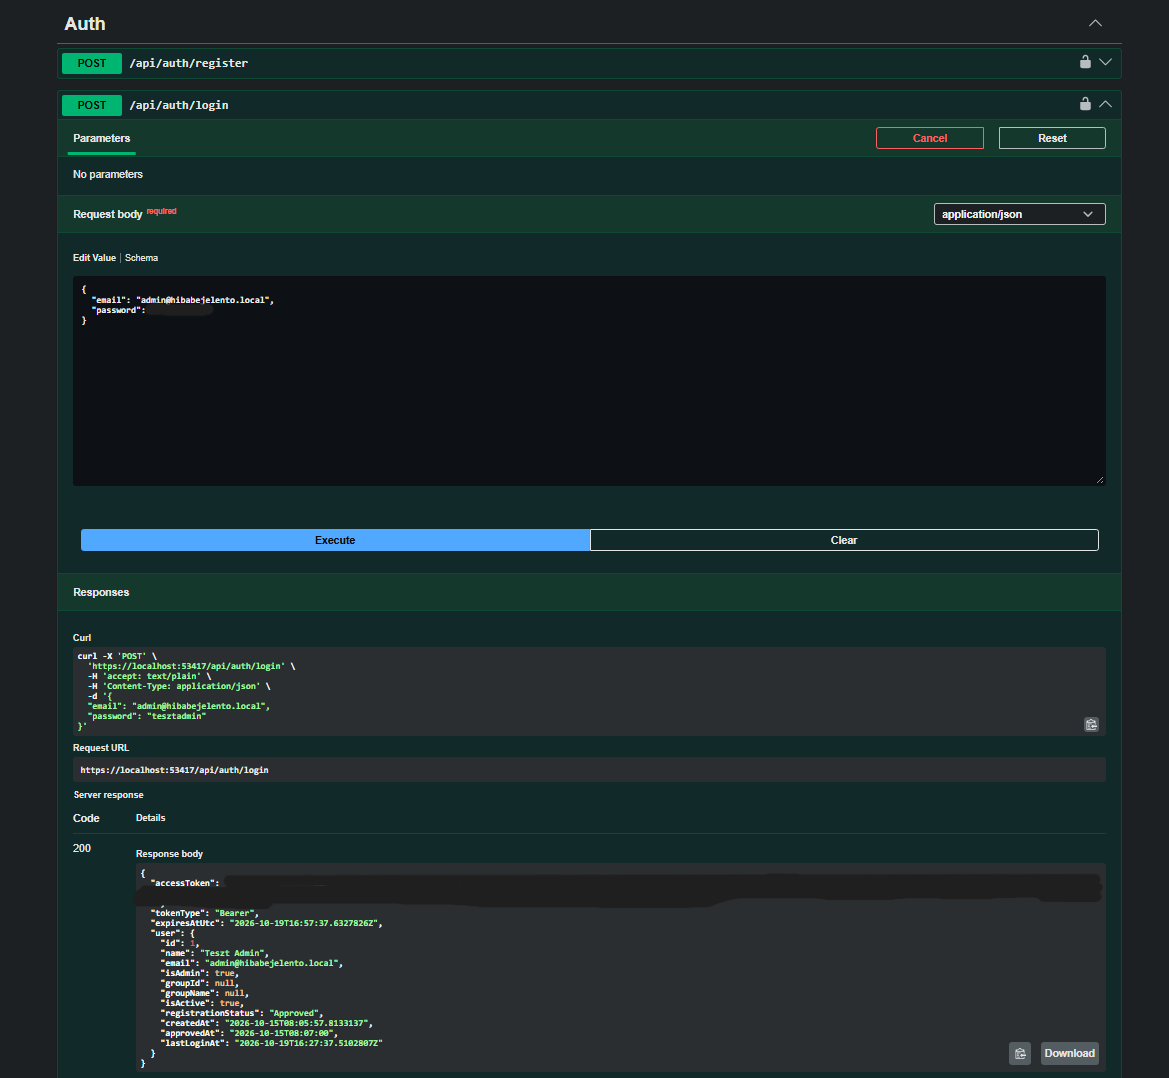
\includegraphics[width=0.95\textwidth,height=0.45\textheight,keepaspectratio]{SwaggerLogin.png}}
        {}
    \caption{Bejelentkezés a Swagger felületén}
    \label{fig:swagger-login}
\end{figure}

\begin{figure}[H]
    \centering
    \IfFileExists{SwaggerAuthorize.png}
        {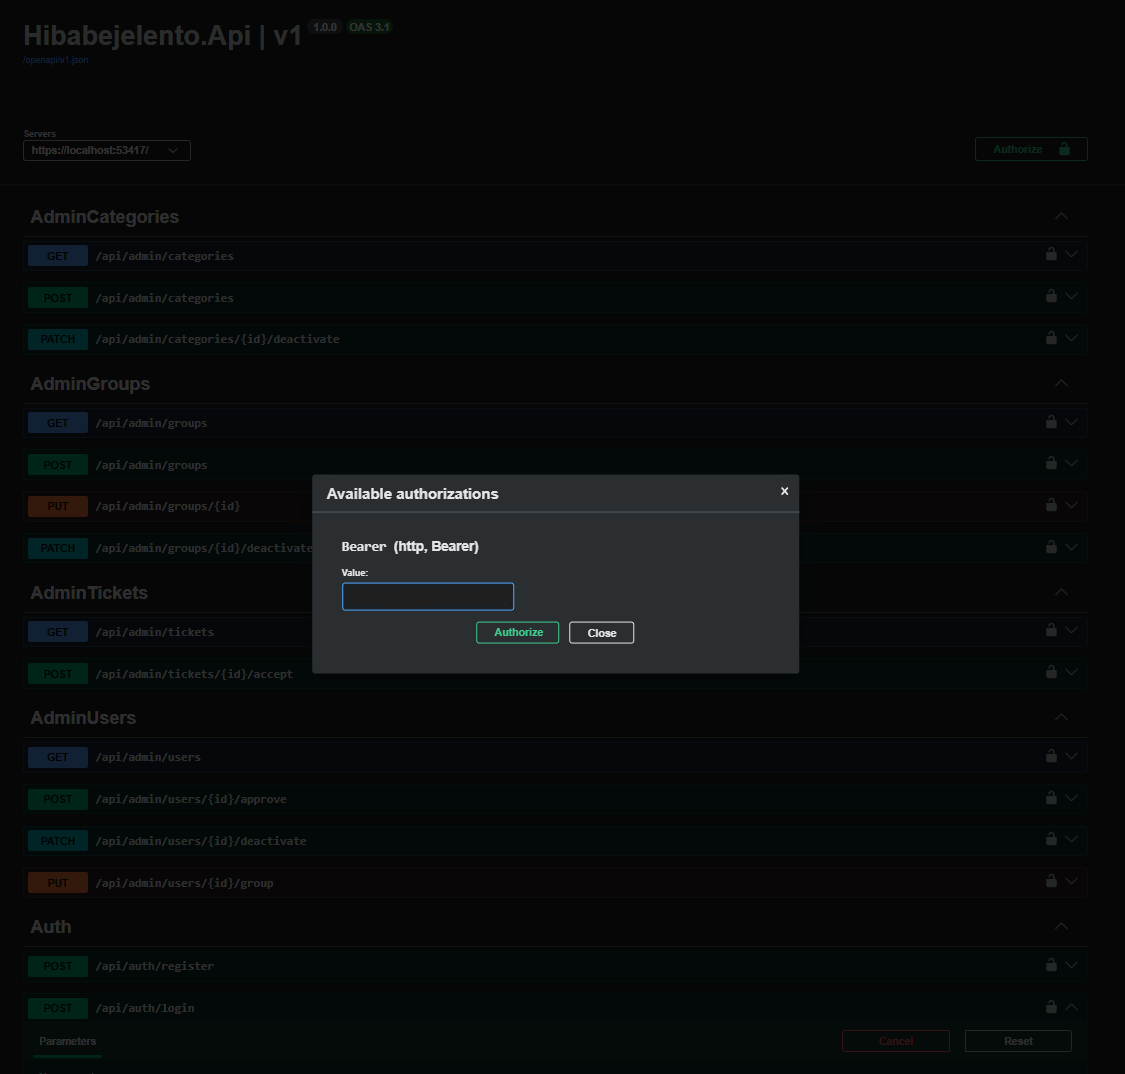
\includegraphics[width=0.95\textwidth,height=0.45\textheight,keepaspectratio]{SwaggerAuthorize.png}}
        {}
    \caption{JWT hozzáadása a Swagger Bearer hitelesítéséhez}
    \label{fig:swagger-authorize}
\end{figure}

\begin{figure}[H]
    \centering
    \IfFileExists{SwaggerTickets.png}
        {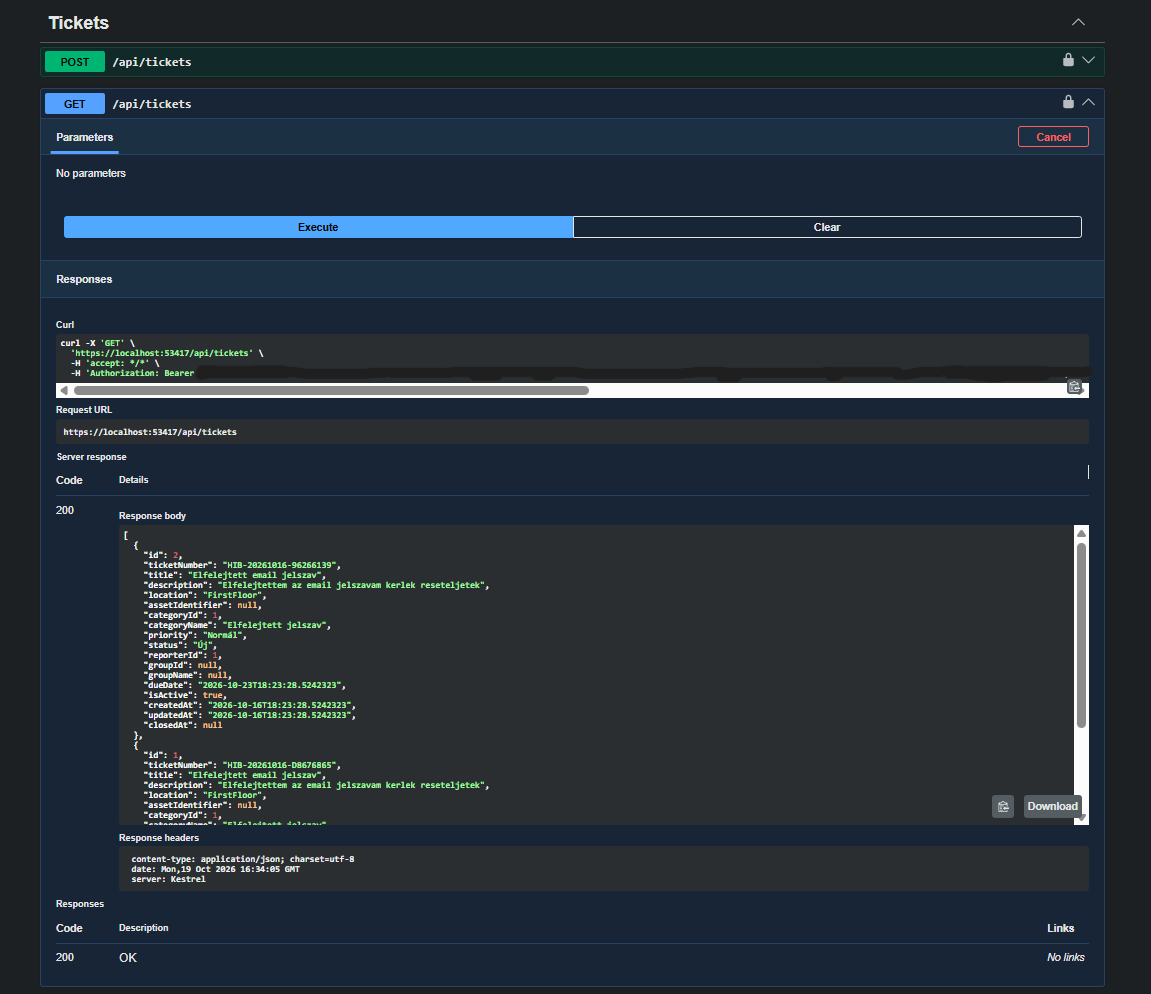
\includegraphics[width=0.95\textwidth,height=0.45\textheight,keepaspectratio]{SwaggerTickets.png}}
        {}
    \caption{A védett ticketlista-végpont sikeres válasza}
    \label{fig:swagger-tickets}
\end{figure}

\subsection{A bejelentés megvalósított életciklusa}

A hibajegy életciklusának minden lépése megvalósult a backendben. A \ref{fig:ticket-states}. ábra az állapotokat és az azokat kiváltó műveleteket mutatja.

\begin{figure}[H]
    \centering
    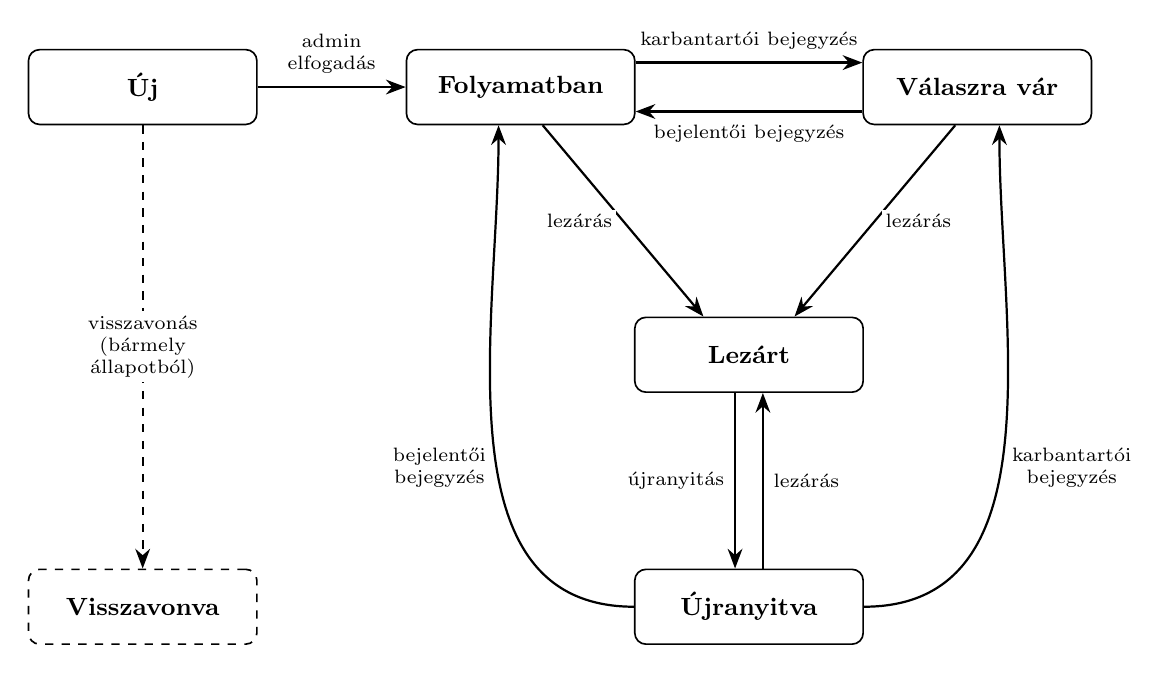
\begin{tikzpicture}[
        state/.style={
            draw=black,
            line width=0.6pt,
            rounded corners=4pt,
            align=center,
            font=\small\bfseries,
            minimum width=2.9cm,
            minimum height=0.95cm
        },
        arrow/.style={-{Stealth[length=2.5mm]}, thick},
        lbl/.style={font=\scriptsize, align=center, fill=white, inner sep=1.5pt}
    ]
        \node[state] (new) at (0,0) {Új};
        \node[state] (prog) at (4.8,0) {Folyamatban};
        \node[state] (wait) at (10.6,0) {Válaszra vár};
        \node[state] (closed) at (7.7,-3.4) {Lezárt};
        \node[state] (reopen) at (7.7,-6.6) {Újranyitva};
        \node[state, dashed] (withdrawn) at (0,-6.6) {Visszavonva};

        \draw[arrow] (new) -- node[lbl, above=3pt] {admin\\elfogadás} (prog);
        \draw[arrow] (prog.12) -- node[lbl, above=3pt] {karbantartói bejegyzés} (wait.168);
        \draw[arrow] (wait.192) -- node[lbl, below=3pt] {bejelentői bejegyzés} (prog.348);
        \draw[arrow] (prog.300) -- node[lbl, left=2pt] {lezárás} (closed.140);
        \draw[arrow] (wait.240) -- node[lbl, right=2pt] {lezárás} (closed.40);
        \draw[arrow] (closed.250) -- node[lbl, left=2pt] {újranyitás} (reopen.110);
        \draw[arrow] (reopen.70) -- node[lbl, right=2pt] {lezárás} (closed.290);
        \draw[arrow] (reopen.west) to[out=180, in=270]
            node[lbl, pos=0.45, left=2pt] {bejelentői\\bejegyzés} (prog.240);
        \draw[arrow] (reopen.east) to[out=0, in=270]
            node[lbl, pos=0.45, right=2pt] {karbantartói\\bejegyzés} (wait.300);
        \draw[arrow, dashed] (new) -- node[lbl] {visszavonás\\(bármely\\állapotból)} (withdrawn);
    \end{tikzpicture}
    \caption{A hibajegy állapotai és az állapotváltozást kiváltó műveletek}
    \label{fig:ticket-states}
\end{figure}

\textbf{Létrehozás és elfogadás.} A létrehozás és az adminisztrátori elfogadás a \ref{sec:states}. alfejezetben leírt módon történik: az \textit{Új} ticket az elfogadással kap csoportot, végleges kategóriát és prioritást, és \textit{Folyamatban} állapotba kerül.

\textbf{Karbantartói felvétel.} A csoport tagja a csoporthoz rendelt, aktív, \textit{Folyamatban} állapotú és még fel nem vett ticketet veheti fel. A felvétel a ticket \texttt{AssignedUserId} mezőjébe írja a karbantartó azonosítóját, az állapot nem változik.

A felvétel egyetlen feltételes adatbázis-utasítással történik: a frissítés csak akkor hajtódik végre, ha a ticket a frissítés pillanatában is fel nem vett és \textit{Folyamatban} állapotú. Ha két karbantartó szinte egyszerre próbálja felvenni ugyanazt a ticketet, az egyik frissítés sikerül, a másik nulla sort módosít, és a backend \texttt{409 Conflict} választ ad. Így nem fordulhat elő, hogy a második kérés felülírja az első felvételt.

\begin{verbatim}
var updatedRows = await _db.Tickets
    .Where(t => t.Id == id
             && t.GroupId == access.GroupId
             && t.IsActive
             && t.Status == TicketStatus.Folyamatban
             && t.AssignedUserId == null)
    .ExecuteUpdateAsync(s => s
        .SetProperty(t => t.AssignedUserId, (int?)userId)
        .SetProperty(t => t.UpdatedAt, now));
\end{verbatim}

\textbf{Bejegyzések és automatikus státuszkezelés.} Bejegyzést a ticket bejelentője és felvevője írhat. A backend a bejegyzés mentésével azonos tranzakcióban állítja be az új állapotot: a karbantartó bejegyzése után \textit{Válaszra vár}, a bejelentőé után \textit{Folyamatban} lesz a ticket. Ha az állapot ténylegesen megváltozott, a változás okával együtt státuszelőzmény-rekord keletkezik. \textit{Új} állapotú ticketen a bejelentő bejegyzése nem módosít az állapoton, így az elfogadás előtti kiegészítés nem kerüli meg az adminisztrátori lépést.

\textbf{Lezárás.} A lezárást csak a ticketet felvevő karbantartó végezheti, aktív, \textit{Folyamatban}, \textit{Válaszra vár} vagy \textit{Újranyitva} állapotú ticketen. A lezárás egy műveletben három dolgot rögzít: a lezárási típussal ellátott végső bejegyzést, a ticket \textit{Lezárt} állapotát a lezárás idejével, valamint a lezárási típust tartalmazó státuszelőzményt. A lezárt ticket aktív marad, ezért a bejelentő később újranyithatja.

\textbf{Újranyitás.} A bejelentő az aktív, \textit{Lezárt} ticketet indoklással újranyithatja. A ticket \textit{Újranyitva} állapotba kerül, a lezárás időpontja törlődik, az indoklás bejegyzésként és a státuszelőzmény okaként is tárolódik. A ticket felvevője nem változik, így a karbantartó a korábbi kommunikáció ismeretében folytathatja a munkát, és a ticket újra lezárható.

\textbf{Visszavonás.} A bejelentő saját hibajegyét állapottól függetlenül visszavonhatja. A visszavonáskor a ticket \textit{Visszavonva} állapotba kerül, inaktívvá válik, megkapja a lezárás időpontját, és a backend rögzíti az állapotváltozás előzményét. A visszavont ticketen további művelet nem végezhető: bejegyzés nem írható hozzá, nem vehető fel és nem nyitható újra.

\subsection{Értesítések kezelése}

Az értesítések célja, hogy a felhasználók észrevegyék a számukra fontos változásokat, például a \textit{Válaszra vár} állapotot vagy egy újranyitott ticketet. Az alkalmazáson belüli értesítések kezelése és az értesítési API-végpontok még hátralévő fejlesztési feladatok. Az értesítések előállításához szükséges események a \texttt{TicketNotes} és a \texttt{TicketStatusHistory} táblában már rendelkezésre állnak. E-mailes értesítés jelenleg nem része a követelményeknek.

\section{Megvalósítás menete és tesztelés}

\subsection{A backend jelenlegi állapota}

A backend ASP.NET Core Web API-ként, .NET 10 célkeretrendszerrel készült. SQLite-adatbázist kezel Entity Framework Core segítségével, a sémaváltozásokat migrációk írják le. A fejlesztői környezet OpenAPI- és Swagger-felületet biztosít.

A megvalósított hitelesítési folyamat tartalmazza a regisztrációt, a jóváhagyott felhasználók bejelentkezését, a JWT hozzáférési token előállítását és ellenőrzését, valamint a bejelentkezett felhasználó adatainak lekérését. A védett kéréseknél a backend ellenőrzi a token érvényességét és a felhasználói fiók aktuális állapotát.

A korábbi állapothoz képest elkészült a karbantartói jegyfelvétel, a saját és a csoportjegyek külön listázása, a bejelentő és a felvevő karbantartó közötti bejegyzések, az ezekhez kötött automatikus státuszkezelés, a lezárási típussal történő karbantartói lezárás, az indoklással történő újranyitás, a státusztörténet lekérdezése, a helyszínek és prioritások adminisztrációja, valamint a visszavonás pontosítása, amely szerint a bejelentő bármikor visszavonhatja saját jegyét. Az értesítési rendszer és a bővített keresés továbbra is hátralévő feladat.

A fejlesztés során a MAUI-kliensből indított ticketlista-kérés \texttt{200 OK} választ adott, amely a felhasználó hibajegyeit tartalmazta. Ez igazolja, hogy az adott próba során a kliens elérte a végpontot, a hitelesítés sikerült, és a backend visszaadta a felhasználó számára látható adatokat.

\begin{figure}[H]
    \centering
    \IfFileExists{AdatbazisBrowser.png}
        {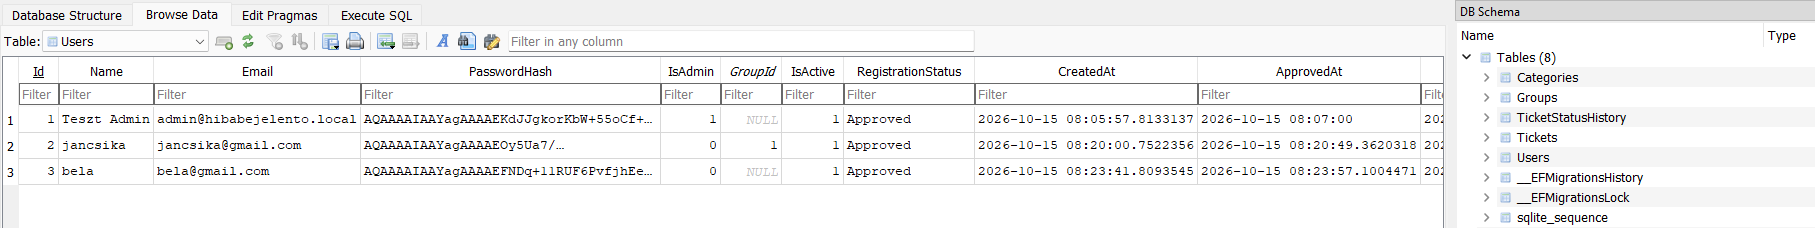
\includegraphics[width=0.95\textwidth,height=0.45\textheight,keepaspectratio]{AdatbazisBrowser.png}}
        {}
    \caption{Az SQLite-adatbázis megtekintése adatbázis-kezelő eszközben}
    \label{fig:database-browser}
\end{figure}

\subsection{A backend indítása fejlesztői környezetben}

A backend indításához .NET 10 SDK szükséges. Az adatbázis-kapcsolat alapértelmezése az \texttt{appsettings.json} fájlban található (\texttt{Data Source=hibabejelento.db}), így külön adatbázisszerver telepítésére nincs szükség. A JWT-beállításokat a projekt mappájában User Secretsként kell megadni:

\begin{verbatim}
dotnet user-secrets set "Jwt:Issuer" "Hibabejelento.Api"
dotnet user-secrets set "Jwt:Audience" "Hibabejelento.Client"
dotnet user-secrets set "Jwt:SigningKey" "<legalább 32 bájtos titkos kulcs>"
dotnet user-secrets set "Jwt:LifetimeMinutes" "30"
dotnet run
\end{verbatim}

Induláskor az alkalmazás automatikusan lefuttatja a hiányzó migrációkat, így friss gépen az adatbázisfájl és a kezdeti prioritások is létrejönnek. A kategóriákat, helyszíneket és csoportokat az adminisztrátornak kell létrehoznia, mielőtt a felhasználók ticketet rögzíthetnének. Az első adminisztrátor kijelölése jelenleg közvetlen adatbázis-módosítással történik.

\subsection{Javasolt fejlesztési sorrend}

A korábbi fejlesztési tervből elkészült a helyszínek és prioritások adminisztratív kezelése, a karbantartói felvétel, a kommunikációs bejegyzések, az automatikus státuszváltás, a karbantartói lezárás, az újranyitás és a státuszelőzmények lekérdezése. A hátralévő feladatok:

\begin{enumerate}
    \item a karbantartói és adminisztrátori felület elkészítése a kliensben, a meglévő végpontokra építve;
    \item a bejegyzések és a státuszelőzmények megjelenítése a hibajegy részletes nézetében;
    \item az alkalmazáson belüli értesítések és a kapcsolódó API-végpontok elkészítése;
    \item szerveroldali keresés és szűrés kategória, prioritás, állapot és dátum szerint;
    \item a bejelentő nevének felvétele a ticket válaszobjektumába;
    \item az ismétlődő vezérlőlogika szolgáltatásosztályba szervezése;
    \item az API automatizált tesztjeinek elkészítése.
\end{enumerate}

A kliensoldali képernyők fejlesztése során minden funkciót össze kell kapcsolni a megfelelő API-végponttal. A képernyőknek kezelniük kell a betöltési állapotot, az üres eredményt, a sikertelen kérést és a szerver által visszaküldött validációs hibát is.

\subsection{Tesztelési terv}

A tesztelés célja annak ellenőrzése, hogy az egyes funkciók a meghatározott követelmények szerint működnek, és hogy a jogosulatlan vagy hibás műveleteket a rendszer megfelelően kezeli. A teszteseteket szerepkörönként és felhasználói folyamatonként célszerű összeállítani.

A tervezett tesztelési területek a következők:

\begin{itemize}
    \item \textbf{API elérhetősége:} az állapotellenőrző végpont elérhető, és helyesen jelzi az adatbázis-kapcsolat eredményét.
    \item \textbf{Regisztráció és jóváhagyás:} a jóváhagyásra váró felhasználó nem fér hozzá védett funkciókhoz, a jóváhagyott felhasználó pedig be tud jelentkezni.
    \item \textbf{JWT-hitelesítés:} token nélkül, hibás tokennel és lejárt tokennel a védett végpontok elutasítják a kérést; érvényes tokennel a hozzáférés sikeres. Az inaktivált felhasználó még érvényes tokenje is elutasításra kerül.
    \item \textbf{Jogosultságok:} a bejelentő nem tekintheti meg más felhasználó bejelentéseit; adminisztratív műveletet csak adminisztrátor végezhet.
    \item \textbf{Bejelentés létrehozása:} a kötelező mezők ellenőrzése, inaktív helyszín és kategória elutasítása, az egyedi azonosító létrehozása és az alapértelmezett prioritás beállítása.
    \item \textbf{Bejelentés láthatósága:} a \texttt{/mine} csak a saját ticketeket, a \texttt{/maintenance} csak a csoport ticketjeit adja vissza; csoporttagság nélkül \texttt{403}.
    \item \textbf{Adminisztratív elfogadás:} az új hibajegy elfogadása, csoporthoz rendelése, kategória- és prioritásbeállítása, a határidő újraszámolása.
    \item \textbf{Felvétel:} csak \textit{Folyamatban} állapotú, fel nem vett ticket vehető fel; a második felvételi kísérlet \texttt{409} választ ad.
    \item \textbf{Bejegyzések:} üres és 5000 karakternél hosszabb bejegyzés elutasítása; csoporttag, aki nem felvevő, nem írhat; az állapot a szerző szerint változik.
    \item \textbf{Lezárás:} csak a felvevő zárhat; érvénytelen lezárási típus és üres végső bejegyzés elutasítása.
    \item \textbf{Újranyitás:} csak a bejelentő nyithat újra, csak lezárt ticketet, indoklás megadásával.
    \item \textbf{Visszavonás:} a bejelentő bármely állapotban visszavonhatja saját hibajegyét; más felhasználó hibajegyét nem vonhatja vissza; visszavont ticketre nem írható bejegyzés.
    \item \textbf{Prioritások:} az alapértelmezett prioritás nem inaktiválható, és mindig pontosan egy aktív alapértelmezett prioritás marad.
    \item \textbf{Hibás bemenet:} üres vagy hibás adatok esetén a rendszer visszautasítja a műveletet, és megfelelő HTTP-státuszkódot ad.
\end{itemize}

A \ref{tab:testcases}. táblázat a teljes ticketfolyamat végigvitelének tervezett lépéseit tartalmazza. A forgatókönyv egy bejelentővel, egy csoporttag karbantartóval és egy adminisztrátorral hajtható végre.

\begin{table}[H]
    \centering
    \footnotesize
    \setstretch{1.15}
    \begin{tabular}{>{\raggedright\arraybackslash}p{0.5cm}>{\raggedright\arraybackslash}p{6.4cm}>{\raggedright\arraybackslash}p{7.6cm}}
        \toprule
        \textbf{\#} & \textbf{Lépés} & \textbf{Várt eredmény} \\
        \midrule
        1 & A bejelentő létrehoz egy ticketet. & \texttt{201}; \textit{Új} állapot, alapértelmezett prioritás. \\
        2 & A karbantartó megpróbálja felvenni. & \texttt{404}, mert a ticket még nincs csoporthoz rendelve. \\
        3 & Az admin elfogadja, csoportot és prioritást ad. & \texttt{204}; \textit{Folyamatban}, új határidő. \\
        4 & A karbantartó felveszi a ticketet. & \texttt{200}; a válaszban a felvevő neve szerepel. \\
        5 & A karbantartó bejegyzést ír. & \texttt{201}; az állapot \textit{Válaszra vár}. \\
        6 & A bejelentő válaszol. & \texttt{201}; az állapot \textit{Folyamatban}. \\
        7 & A karbantartó 1-es típussal lezárja. & \texttt{200}; \textit{Lezárt}, kitöltött lezárási idő. \\
        8 & A bejelentő bejegyzést próbál írni. & \texttt{409}, lezárt tickethez nem írható bejegyzés. \\
        9 & A bejelentő indoklással újranyitja. & \texttt{200}; \textit{Újranyitva}, a felvevő változatlan. \\
        10 & A bejelentő visszavonja. & \texttt{204}; \textit{Visszavonva}, inaktív ticket. \\
        11 & A státuszelőzmények lekérése. & Minden állapotváltozás időrendben, indokkal. \\
        \bottomrule
    \end{tabular}
    \caption{A teljes ticketfolyamat tervezett tesztforgatókönyve}
    \label{tab:testcases}
\end{table}

A tesztelés során rögzíteni kell a teszt lépéseit, a várt eredményt és a tényleges eredményt. A dokumentációban csak ténylegesen lefuttatott tesztek eredménye szerepelhet kész eredményként; a még le nem futtatott eseteket tesztelési tervként kell megjelölni.

\subsection{Ismert korlátok és továbbfejlesztési lehetőségek}

A backend hitelesítési, jogosultság-ellenőrzési, hibajegy-életciklus és adminisztrációs végpontjai elkészültek. Az ismert korlátok:

\begin{itemize}
    \item Az alkalmazáson belüli értesítések még nem készültek el.
    \item A keresés szerveroldalon csak a pontos ticketazonosító alapján működik; a részleges szöveges keresés és a részletes szűrés -- például állapot, kategória, prioritás és dátum szerint -- későbbi bővítés.
    \item A határidő-számítás nem veszi figyelembe a munkaszüneti napokat, és a prioritás határidejének módosítása nem hat a meglévő ticketekre.
    \item A ticket válaszobjektuma nem tartalmazza a bejelentő nevét, ezért a kliens jelenleg az azonosítóját jeleníti meg.
    \item Az adminisztrátor a ticketek bejegyzéseit nem látja, csak a státuszelőzményeket.
    \item Az inaktivált csoport, kategória, helyszín és prioritás újraaktiválására nincs végpont.
    \item A státuszelőzmény indokának oszlopa 500 karakteres korláttal van definiálva, az újranyitás indoklása viszont 5000 karakter is lehet. SQLite alatt ez nem okoz hibát, mert az adatbázismotor nem kényszeríti ki a szöveghosszt, de más adatbázismotorra váltás előtt össze kell hangolni a két korlátot.
    \item Az első adminisztrátor csak közvetlen adatbázis-módosítással hozható létre.
    \item A CORS-beállítás jelenleg minden forrást engedélyez, ami fejlesztéshez megfelelő, éles üzemhez szigorítani kell.
    \item Automatizált tesztek még nem készültek.
\end{itemize}

További fejlesztési lehetőség a csatolmányok kezelése, részletesebb statisztikák és külső értesítési csatorna bevezetése. Ezek nem részei az első változat minimális funkcióinak.

\section{Összegzés}

A projekt célja egy olyan asztali hibabejelentő és karbantartás-kezelő rendszer megtervezése és megvalósítása, amelyben a felhasználók rögzíthetik a problémákat, a karbantartók kezelhetik azokat, az adminisztrátor pedig felügyelheti a rendszer működését. A csapat a kiírás általános műszaki hibakezelési feladatát vállalati IT-infrastruktúrára szűkíti.

A rendszer .NET MAUI kliensből, .NET Web API-ból és szerveroldali SQLite-adatbázisból áll. A backend Entity Framework Core-t használ az adatkezeléshez. A megvalósított szerveroldali funkciók lefedik a hibajegy teljes életciklusát: a létrehozást, az adminisztrátori elfogadást, a karbantartói felvételt, a bejelentő és a karbantartó közötti bejegyzéseket, az ezekhez kötött automatikus státuszkezelést, a típus szerinti lezárást, az újranyitást és a visszavonást. Minden állapotváltozás előzményként tárolódik. Az adminisztrátor a felhasználók és csoportok mellett a kategóriákat, helyszíneket és prioritásokat is kezeli.

A kliensben a bejelentkezés, a hibajegylista keresése és szűrése, a hibajegy adatainak megjelenítése és új hibajegy létrehozása érhető el. A fejlesztői Swagger felületen a védett végpontok Bearer tokennel próbálhatók ki. A következő lépések a karbantartói és adminisztrátori kliensfelület, az értesítési rendszer, a bővített keresés és az automatizált tesztek elkészítése.

\newpage
\clearpage

\renewcommand{\bibsection}{}

\begin{center}
    \noindent
    {\headingFont\bfseries\fontsize{16}{24}\selectfont Irodalomjegyzék}
\end{center}
\addcontentsline{toc}{section}{Irodalomjegyzék}
\vspace{12pt}

\bibliographystyle{apalike}
\bibliography{references}

\end{document}
